
%--------------------------------------------------------------------------
\chapter{INTRODUCTION}

\vspace{3em}
\setlength{\epigraphwidth}{0.86\textwidth}
\setlength{\epigraphrule}{0pt}
\epigraph{
	\textit{Music has become an almost arbitrary matter, and composers will no longer be bound by laws and rules, but avoid the names of School and Law as they would Death itself...}
}{\vspace{2em}-- Johann Joseph Fux}
\vspace{1em}

\begin{figure}[htbp]
    \centering
	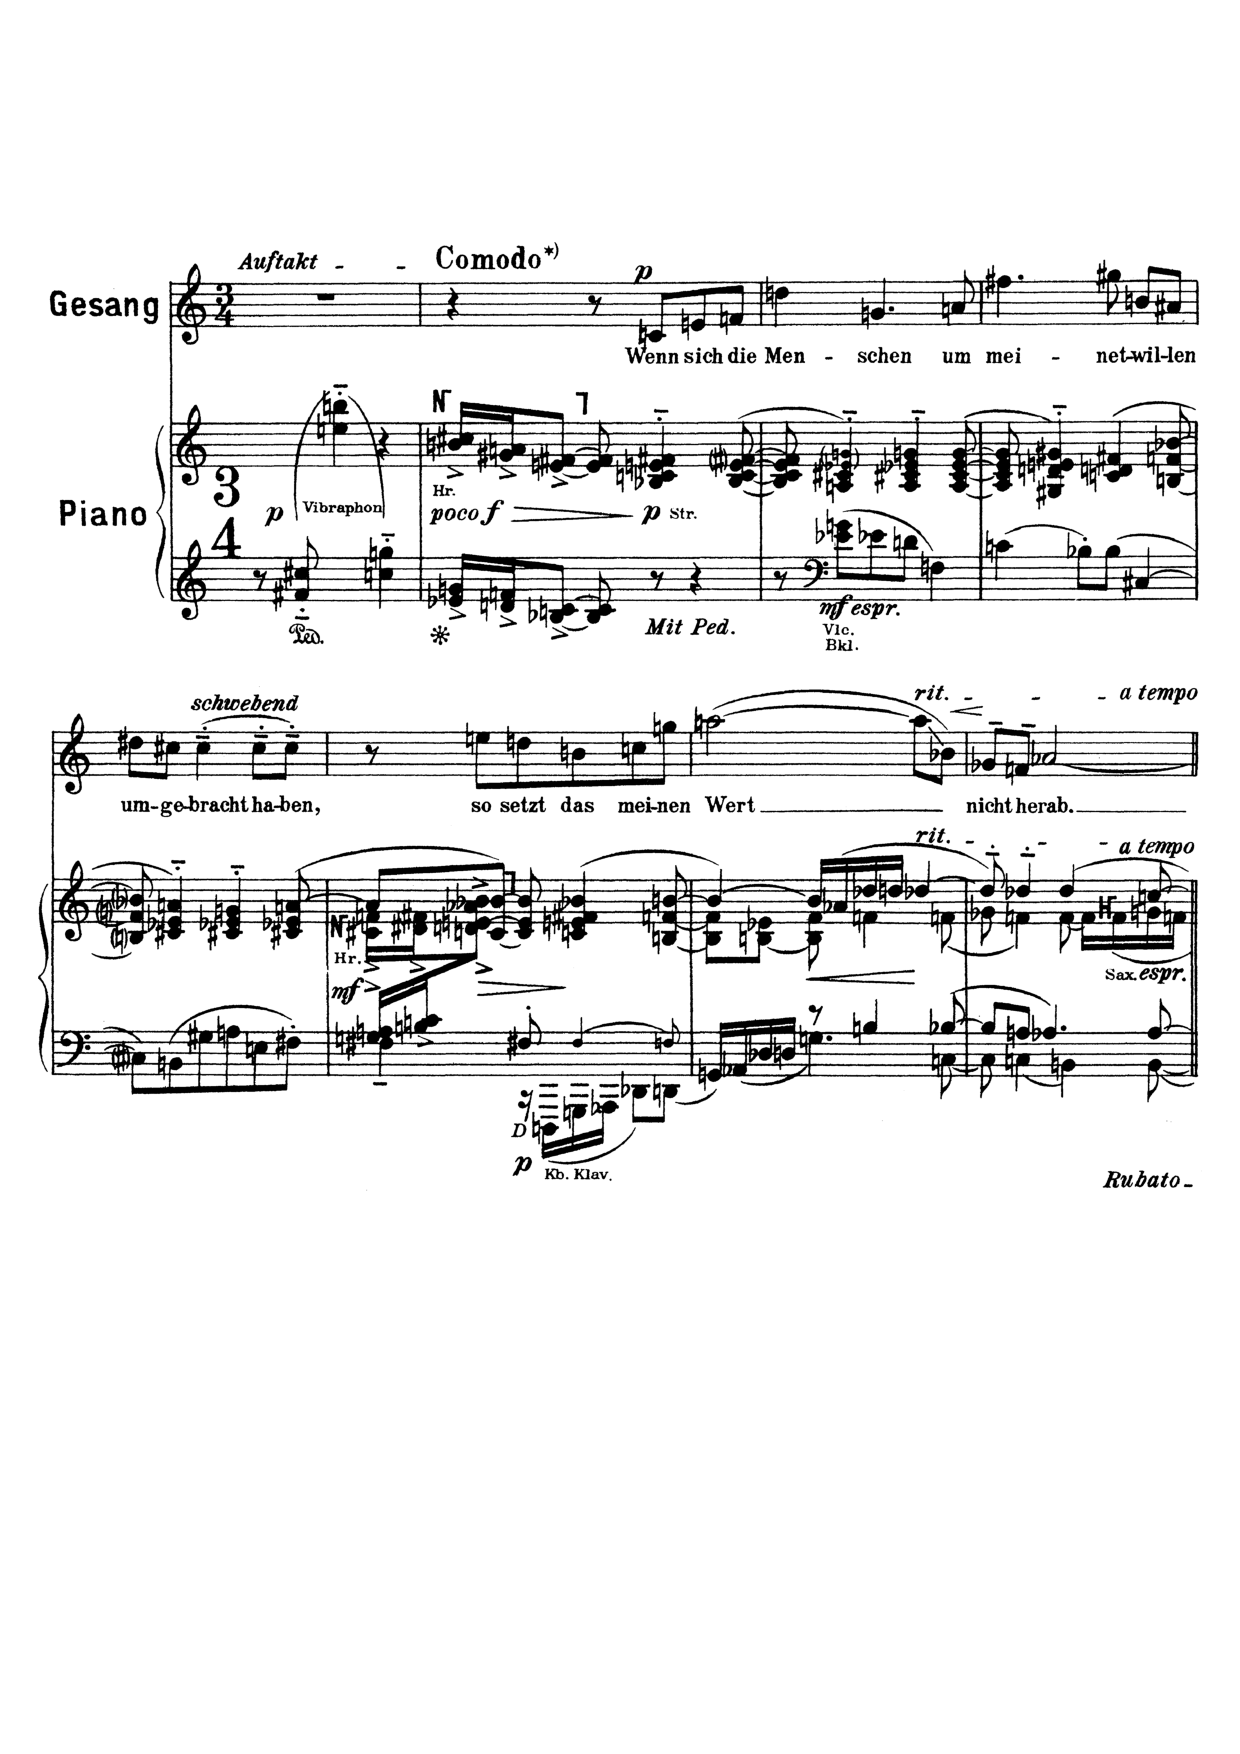
\includegraphics[width=6.5in]{figures/berg1.pdf}
	\caption[Berg's \emph{Lulu}]{Alban Berg's \emph{Lulu} \cite[182]{Starr1984}.}
	\label{fig:berg-lulu}
\end{figure}

%--------------------------------------------------------------------------
\section{Basic Derivation Theory}

Derivation is the process of extracting ordered segments from rows in order to generate new compositional materials. It is a technique that dates back to the Second Viennese School. In its most incipient form, a composer may simply extract these segments from a row, and combine them to form another, as we see in Berg's \emph{Lulu}. The basic row used by Berg is $S = \{ 10, 2, 3, 0, 5, 7, 4, 6, 9, 8, 1, 11 \}$. In the Prologue, however, one is greeted with the row $\{ 10, 3, 4, 9, 2, 7, 8, 1, 0, 5, 6, 11 \}$, as depicted in Fig.~\ref{fig:berg-prologue}. It is clear that the segments that constitute the Prologue's row are ordered segments in the basic row form, and the fact that one row cannot obtained from another via row operations is here irrelevant.

\begin{figure}[htbp]
    \centering
	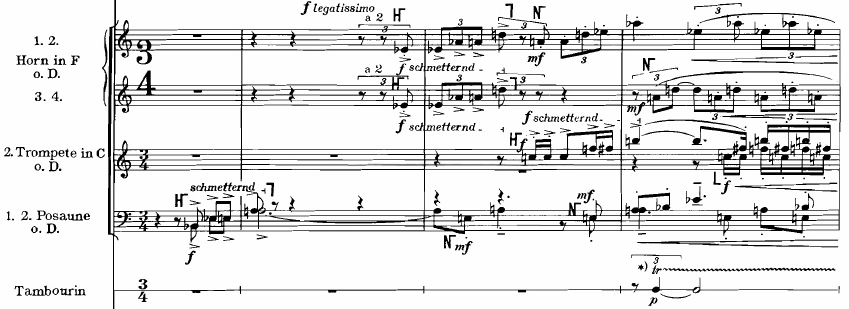
\includegraphics[width=6.5in]{figures/berg2.png}
	\caption[Derived Row in Berg's \emph{Lulu}]{Derived row in the \emph{Prologue} of Alban Berg's \emph{Lulu} \cite[182]{Starr1984}.}
	\label{fig:berg-prologue}
\end{figure}

Less naive approaches to derivation often involve a derived row that will have more structure. In them, one will usually see a combination matrix where derived and original rows are matched with some twelve-tone or order operation of themselves, or both. This is illustrated in Ex.~\ref{ex:derivation}.

\begin{example}
	\label{ex:derivation}
	We may use the basic row in \emph{Lulu} as motivation for a basic derivation procedure. The first step is to create a $2 \times 24$ array where the first row is $S$ followed by $\R(S)$, and the second row is initially undefined.
	\begin{equation}
    	\left[
    	\begin{array}{cccccccccccc|cccccccccccc}
        	10 & 2 & 3 & 0 & 5 & 7 & 4 & 6 & 9 & 8 & 1 & 11 & 11 & 1 & 8 & 9 & 6 & 4 & 7 & 5 & 0 & 3 & 2 & 10 \\
        	. & . & . & . & . & . & . & . & . & . & . & . & . & . & . & . & . & . & . & . & . & . & . & .
    	\end{array}
    	\right] \enspace.
	\end{equation}
	Next, one chooses an arbitrary segment, and separates it from the the top row by placing in in the bottom row:
	\begin{equation}
    	\left[
    	\begin{array}{cccccccccccc|cccccccccccc}
        	. & 2 & 3 & . & . & . & 4 & 6 & 9 & 8 & 1 & 11 & . & . & . & . & . & . & 7 & 5 & 0 & . & . & 10 \\
        	10 & . & . & 0 & 5 & 7 & . & . & . & . & . & . & 11 & 1 & 8 & 9 & 6 & 4 & . & . & . & 3 & 2 & .
    	\end{array}
    	\right] \enspace.
	\end{equation}
	Let $V = \{ 2, 3, 4, 6, 9, 8, 1, 11, 7, 5, 0, 10 \}$. Then $V$ is a row derived from $S$. In particular, the ordered segment $\{ 10, 0, 5, 7 \}$ in $S$ is preserved by $\R(V)$, and a counterpoint that combines $S$ vertically with $V$ horizontally is possible by construction.
\end{example}

It is of interest to note at this point that, in this kind of construction, the choice of a particular segment is already an important compositional decision. This choice bears relevance in that it establishes motivic material, that is, the segment itself. It also potentially introduces complementary harmonic regions, one given by the segment, the other given by its set complement. Moreover, and perhaps more importantly, it presents an opportunity for exploring syntax. There are a multitude of ways in which a composer may obtain syntax from a simple derivation procedure such as the one given in the example above. One way would be to find an operation that makes the chosen segment invariant. In particular, it is easily checked that $S_1 = \{ 10, 0, 5, 7 \} = \R\T_5\I(S_1)$. One can then extend Ex.~\ref{ex:derivation} into the combination array $[S \; | \; \R(S) \; | \; \R\T_5\I(S) \; | \; \T_5\I(S_1)]$. In the extended array, the segment $S_1$ would be preserved, but the row derived from $\R\T_5\I(S)$ would not be a transform of $V$. If the set complement of $S_1$ in $V$ were parsed to produce more than one harmonic region, then the complement of $S_1$ under this new derived row would produce different harmonic regions. This can be very pertinent compositionally, as one would be capable of producing contrasting harmonic regions while maintaining motivic coherence under the $S_1$ segment.

Yet another way of generating syntax from derivation would be to follow $S$ with $V$ itself. One would then derive a new row from $V$, say $Q$, and eventually follow $V$ with $Q$. Repeating this procedure \emph{ad libitum} could generate many contrasting harmonic regions. In particular, this type of derivation is seen in Donald Martino's \emph{Notturno} of 1974, a composition that won the Pulitzer Prize in the following year \cite[181]{Starr1984}. If, by compositional choice, the chain of derived rows picked always the same order numbers, then a potential for rhythmic and agogic coherence could also be explored.

The beginnings of derivation techniques can be traced back to Donald Martino's \emph{The Source Set and Its Aggregate Formations} \cite{Martino1961}, a paper whose main purpose is another, namely to generalize the construction of columnar realizations, although this latter term appears to have been coined by \cite{Starr1984}. The techniques employed by Martino are heavily influenced by Babbitt's ideas on combinatoriality \cite[224]{Martino1961}, and make extensive use of tables. Below is a fragment of the source hexachords table given in \cite[229]{Martino1961}. The author, in the interest of generalizing the procedure, provides also trichordal, tetrachordal, and even pentachordal combinatoriality tables, as well as a somewhat brief discussion on uneven partitions of a row and their combinatoriality implications \cite[267]{Martino1961}.

\begin{table}[htbp]
    \caption[Martino's Source Hexachords]{Fragment of a table for consulting source hexachords in \cite[229]{Martino1961}.}
    \centering
    \vspace{12pt}
    \begin{tabular}{c|cccccc}
        \hline\\
        No. & Set & Interval Vector & TTO's \\\\
        \hline\\
        A1 & $\{0,1,2,3,4,5\}$ & $\langle 5,4,3,2,1,0 \rangle$ & $\{\T_6,\T_{11}\I,\R\T_{11},\R\T_6\I\}$ \\\\
        B2 & $\{0,2,3,4,5,7\}$ & $\langle 3,4,3,2,3,0 \rangle$ & $\{\T_6,\T_{1}\I,\R\T_{1},\R\T_6\I\}$ \\\\
        3 & $\{0,1,3,4,5,8\}$ & $\langle 3,2,3,4,3,0 \rangle$ & $\{\T_6,\R\T_2\}$ \\\\
        E4 & $\{0,1,4,5,8,9\}$ & $\langle 3,0,3,6,3,0 \rangle$ & $\{\T_{2,6,10},\T_{3,7,11}\I,\R\T_{3,7,11},\R\T_{2,6,10}\I\}$ \\\\
        C5 & $\{0,2,4,5,7,9\}$ & $\langle 1,4,3,2,5,0 \rangle$ & $\{\T_6,\T_{3}\I,\R\T_{3},\R\T_6\I\}$ \\\\
        \hline
    \end{tabular}
\end{table}

Martino acknowledges the aggregates formed by combinatoriality are not necessarily ordered \cite[228]{Martino1961}, rather seeing it from the bright side of diversity, in which the set union of a columnar aggregate being capable of \emph{deriving} a different row class is actually more appealing than self-similarity, which is not at all considered. The same passage brings, to our knowledge, the first \emph{explicit} mention in the literature of a technique for deriving new rows from columnar aggregates in more generality than what we see in Schoenberg's fourth string quartet, as seen in \ref{ex:martino-derivation}. In mentioning derivation, Martino juxtaposes it to another, in his view, way of progressing through hexachords, namely the \emph{fragmentation} or partitioning of the original series, ultimately deeming both procedures essentially the same, as derivation via aggregate realizations can surely be seen as the fragmentation of the (new) series obtained vertically.

\begin{example}
	\label{ex:martino-derivation}
	\cite[230]{Martino1961}
	Let $S = \{ 0, 4, 11, 3, 1, 2, 5, 6, 9, 8, 10, 7 \}$ and consider the trivial  combination matrix given below.
	\begin{equation}
    	\hat{A} = [\hat{A}_1 | \hat{A}_2 | \hat{A}_3 | \hat{A}_4] = \left[
    	\begin{array}{ccc|ccc|ccc|ccc}
        	0 & 4 & 11 & 3 & 1 & 2 & 5 & 6 & 9 & 8 & 10 & 7 \\
        	7 & 10 & 8 & 9 & 6 & 5 & 2 & 1 & 3 & 11 & 4 & 0
    	\end{array}
    	\right] \enspace.
	\end{equation}
	In particular, the hexachords given by $\hat{A}_i$ can be combined with their transforms under $\T_1\I$, yielding the following matrix:
	\begin{equation}
    	A = [A_1 | A_2 | A_3 | A_4] = \left[
    	\begin{array}{ccc|ccc|ccc|ccc}
        	0 & 4 & 11 & 3 & 1 & 2 & 5 & 6 & 9 & 8 & 10 & 7 \\
        	7 & 10 & 8 & 9 & 6 & 5 & 2 & 1 & 3 & 11 & 4 & 0 \\
        	\hline
        	1 & 9 & 2 & 10 & 0 & 11 & 8 & 7 & 4 & 5 & 3 & 6 \\
        	6 & 3 & 5 & 4 & 7 & 8 & 11 & 0 & 10 & 2 & 9 & 1
    	\end{array}
    	\right] \enspace.
	\end{equation}
	We can then \textbf{almost} derive transforms of the row $Q = \{ 7, 0, 10, 6, 4, 1, 3, 5, 8, 9, 2, 11 \}$ from the columns of $A$, except for a single symmetry between 6 and 5, as seen below.
	\begin{equation}
        \left[
        \begin{array}{cccccccccccc|cccccccccccc}
            & 0 &&& 4 &&&&&&& 11 &&&& 3 & 1 &&& 2 &&&& \\
            7 && 10 &&&&&& 8 &&& && 9 &&&&&&& \boxed{6} & \boxed{5} && \\
            \hline
            &&&&& 1 &&&& 9 & 2 & &&&&&& 10 & 0 &&&& 11 & \\
            &&& 6 &&& 3 & 5 &&&& & 4 && 7 &&&&&&&&& 8
        \end{array}
        \right. \cdots
    \end{equation}
    This apparent failure did not seem to bother Martino at all, as his focus remained in establishing a concrete foundation for combinatoriality. In order to extend the above procedure to eight rows of counterpoint, some adjustments must be made, namely we need columnar aggregates whose rows are allowed to have different numbers of elements, as seen below. This second folding is otherwise accomplished much the same way, by choosing a hexachord from $A_1$, and determining its combinatoriality properties via table lookup.
    \begin{equation}
    	\left[
    	\begin{array}{cc|cc|cc|cc|}
        	0 & 4 & 11 && 3 & 1 & 2 & \\
        	7 & 10 & 8 && 9 && 6 & 5 \\
        	1 && 9 & 2 & 10 && 0 & 11 \\
        	6 && 3 & 5 & 4 & 7 & 8 & \\
        	2 && 6 & 1 & 5 && 3 & 4 \\
        	9 && 0 & 10 & 11 & 8 & 7 & \\
        	3 & 11 & 4 && 0 & 2 & 1 & \\
        	8 & 5 & 7 && 6 && 9 & 10
    	\end{array}
    	\right. \cdots
	\end{equation}
\end{example}

It is easy to understand why Martino was so motivated by creating as much diversity as possible from a single row in a structured manner. If not because creating variation upon some fixed foundation has been a constant in music composition since Bach, serialism up to that point had seen countless pieces in which the very same series was presented over and over again, frequently in the same $\R\T_n\I$ form for entire passages. As innovative as it is, not even the first movement of Schoenberg's fourth string quartet escapes this paradigm. The idea of having a systematic approach to syntactically moving from one row class to another, although latent in late Schoenberg, ultimately defines one one of the most remarkable trends in the next chapter of serialism. Martino actually manages to solve both problems at once with derivation, as it gives the composer the opportunity to focus on the derived rows, while using a somewhat more abstract row to generate syntax, even though we only see this potential explored in his later pieces, and not quite yet in \cite{Martino1961}. For now, what is most important is to derive as much harmonic diversity from the rigidity of an omnipresent series as possible.

What \cite{Starr1984} terms \emph{skewed polyphonization}, and what we called shifted derivation in Sec.~\ref{shifted-derivation}, has too an origin in what Martino calls, in turn, \emph{oblique combination}. Ex.~\ref{ex:oblique} deals with the tetrachordal case, although other cases, including those where the overlap occurs at unequal partitionings of the row are considered. Similarly to our intuition in Sec.~\ref{shifted-derivation}, oblique combinations are seen as special, yet straightforward cases of other types of combinatoriality \cite[267]{Martino1961}.

\begin{example}
	\cite[241]{Martino1961}
	\label{ex:oblique}
	Let $S = S_1 | S_2 | S_3$ be a twelve-tone row, partitioned into tetrachords. Let $f$ and $g$ be TTO's, and considered the following oblique combination matrix:
	\begin{equation}
    	\left[
    	\begin{array}{c|c|c|c|c}
        	S_1 & S_2 & S_3 & . & . \\
        	. & f(S_3) & f(S_2) & f(S_1) & . \\
        	. & . & g(S_1) & g(S_2) & g(S_3)
    	\end{array}
    	\right] \enspace.
	\end{equation}
	It follows:
	\begin{enumerate}[i.]
		\item If $S_1 = \T_i\I(S_1)$ \textbf{only} for some $i$, then $f = \R\T_j$ for some $j$, and $g = \T_k\I$ for some $k$;
		\item If $S_3 = \T_i\I(S_3)$ \textbf{only} for some $i$, then $f = \R\T_j\I$ for some $j$, and $g = \T_k$ for some $k$;
		\item If $S_1 = \T_i\I(S_1)$ \textbf{only} for some $i$ and $S_3 = \T_j\I(S_3)$ for some $j$, then $f = \R\T_k\I$ for some $k$, and $g = \T_\ell\I$ for some $\ell$;
		\item If $S_1 = \T_i\I(S_1)$ \textbf{only} for some $i$, $S_3 = \T_j\I(S_3)$ for some $j$, and $S_1 = \T_k(S_3)$ for some $k$, then $f = \T_\ell\I$ or $f = \R\T_\ell\I$ for some $\ell$, and $g = \T_m\I$ or $g = \R\T_m\I$ for some $m$;
		\item If $S_1 = \T_i(S_3)$ \textbf{only} for some $i$, then $f = \T_j$ or $f = \R\T_j$ for some $j$, and $g = \T_k$ or $g = \R\T_k$ for some $k$;
		\item If $S_3 = \T_i\I(S_1)$ \textbf{only} for some $i$, then $f = \T_j\I$ or $f = \R\T_j$ for some $j$, and $g = \T_k$ or $g = \R\T_k\I$ for some $k$.
	\end{enumerate}
\end{example}

In one of the seminal academic works in the field of twelve-tone theory, \cite{Starr1984} utilizes a mostly set-theoretic framework to understand and categorize rows and procedures involved in producing derivation, polyphony, and self-derived combination matrices. The main objective is similar to ours, in it has a bias toward unveiling self-derivation, which unfortunately still remains a somewhat obscure topic. The set-theoretic approach revolves around the idea of looking at collections from the standpoint of their order constraints: a totally constrained set with no precedence contradictions is a twelve-tone row; a completely unconstrained set of twelve tones represents the free aggregate; a maximally constrained one is what the author calls the simultaneous aggregate, that is, a twelve-tone cluster. Sets that live in-between can often be projected in the middle and background of a composition, fact that amounts to a Schenkerian-flavored view of the whole process.

Mathematically, the ideas in \cite{Starr1984} translate into considering the set $U$ of all ordered pairs of pitch classes. There are twelve choices for the first position, and twelve choices for the second position. As both choices are independent, this set has cardinality $12^2 = 144$. An element of $U$ is called an order constraint, and a subset $C$ of $U$ is called a pitch-class relation. The latter can be viewed as a $12 \times 12$ matrix where the entry $c_{ij}$ is equal to one whenever $\{ i, j \} \in C$, and zero otherwise. One can then apply bitwise operations to these matrices in a very computationally efficient manner: bitwise \emph{and} and \emph{or} correspond respectively to set intersection and union. For any pair of pitch classes $x$ and $y$, we define a relation $x \sim y$ on the power set of $U$ by the set inclusion of the element $\{ x, y \}$. A subset $C$ will then be reflexive if, whenever an element of $C$ (which is a set) contains the pitch class $x$, then $\{ x, x \} \in C$. In words, reflexivity means that if a reflexive collection $C$ of notes contains an element $x$, then $x$ precedes (and follows) itself in $C$. The free aggregate is a minimal reflexive subset of $U$ that contains all twelve tones. The relation $\sim$ will be symmetric if $\{ x, y \} \in C$ implies $\{ y, x \} \in C$, and antisymmetric whenever $\{ x, y \} \in C$ implies $\{ y, x \} \notin C$, for $x \ne y \in \mathbb{Z}/ 12 \mathbb{Z}$. Similarly, transitivity is defined as $\{ x, y \} \in C$ and $\{ y, z \} \in C$, then $\{ x, z\} \in C$; and trichotomy is defined as either $\{ x, y \} \in C$ or $\{ y, x \} \in C$ for any $x \ne y \in \mathbb{Z}/ 12 \mathbb{Z}$. The relation $\sim$ is, of course, an order relation on the set of twelve tones by definition. A partial order is one that is reflexive, transitive, and antisymmetric, while a total order (a row), is a partial order that satisfies trichotomy.

Often, pitch-class relations will contain many redundancies due to transitivity. In order to express these relations as oriented graphs, one must first remove, or prune, such redundancies. This process can be reversed and a pitch-class relation can be extended to the point of its transitive closure. It is also common for a pitch-class relation to be absent of any order constraint involving both $\{ x, y \}$, in which case we say $x$ and $y$ are incomparable. Such $x$ and $y$ are bound to be struck together, or else be \emph{linearized} by the injection of some constraint that will make them comparable, as long as there remains still a partial order, that is, as long as this process does not introduce a symmetry, for instance. The set of all total orderings that can be linearized out of some partial order is called its total order class. In a completely analogous manner, one can \emph{verticalize} a pitch-class relation by removing constraints, and again minding that the result is still transitive and symmetric. We say a partial order covers another whenever the former is a verticalization of the latter. A simple procedure to guarantee that a verticalization will remain a partial order is to take its union with the free aggregate, then subject this union to an extension operation, thus providing reflexivity in the first step, as well as transitivity in the second. We can say the following about covering, and about unions and intersections of pitch-class relations:

\begin{theorem}
    \cite[193]{Starr1984}
    \begin{enumerate}[i.]
        \item Covering is transitive;
        \item A pitch-class relation is covered by its extension;
        \item If a pitch-class relation covers another, then the extension of the former covers the extension of the latter.
    \end{enumerate}
\end{theorem}

\begin{theorem}
    \cite[194]{Starr1984}
    \label{starr-theorem}
    Let $A$ and $B$ be partial orders and denote by $\Toc(A)$ and $\Toc(B)$ their respective total order classes. Then
    \begin{equation}
        \Toc(A) \cap \Toc(B) = \Toc(\Ext(A \cup B)) \enspace,
    \end{equation}
    where $\Ext$ is the extension operator. Moreover, if $A_i$ is a finite sequence of $n$ partial orders, then
    \begin{equation}
        \bigcap_{i = 0}^{n} \Toc(A_i) = \Toc \left[ \Ext\left ( \bigcup_{i = 0}^{n} A_i \right) \right] \enspace.
    \end{equation}
\end{theorem}

\begin{theorem}
    \cite[194]{Starr1984}
    The intersection of two partial orders is again a partial order.
\end{theorem}

Th.~\ref{starr-theorem} will play a crucial role in the development of derivation techniques. Of vital importance is the fact that one can operate on pitch-class relations the same way one operates on pitch-class sets:

\begin{theorem}
    \cite[195]{Starr1984}
    Let $C$ be a pitch-class relation and $\{ a, b \}$ an element of $U$ such that $\{ a, b \} \in C$.
    \begin{enumerate}[i.]
        \item If $F$ is a pitch-class operation, then $\{ F(a), F(b) \} \in F(C)$ if and only if $\{ a, b \} \in C$. In particular, if $\R(C)$ is the retrograde of $C$, then $\{ a, b \} \in \R(C)$ if and only if $\{ b, a \} \in C$.
        \item If $C$ is totally ordered, then $\R(C) = (S \setminus D) \cup F$, where $S$ is the simultaneous aggregate and $F$ is the free aggregate.
        \item If $C_1$ covers $C_2$, then $F(C_1)$ covers $F(C_2)$.
        \item Finally, if $C$ is $F\R$-invariant, then all cycles in $F$ have length two.
    \end{enumerate}
\end{theorem}

%--------------------------------------------------------------------------
\subsection{Aggregate Realizations}

In this section we will define the important concept of \emph{aggregate realizations}, which will, in turn, lead to a classification of partial orders, as well as to many musical applications. An aggregate realization is a particular type of partial order $C$ in which, for any pair of pitch classes $a, b$, if $a$ and $b$ are incomparable in $C$, then the set of pitch classes that precede $a$ in $C$ is equal to the set of pitch classes that precede $b$ in $C$, and also the set of pitch classes that follow $a$ in $C$ is equal to the set of pitch classes that follow $b$ in $C$. Aggregate realizations arise naturally from a total order in the sense that they belong to the set of all partial orders that are covered by said total order. An interesting compositional application of aggregate realizations is that of projecting a total order as a middle-ground entity.

\begin{example}
    \cite[197]{Starr1984}
    Given a sequence $S$ of partial orders, all of which covered by the same total order, say $X$, if both $X$ is never stated in the foreground and $S$ contains all order constraints in $X$, then a musical passage in which $S$ is stated in the foreground will bear $X$ as a middle-ground entity. In the case where $S$ does not comprise all the order constraints in $X$, some other partial order that covers $S$ will be projected in the middle-ground. In the particular case where a composer is dealing with pitch classes, projecting a partial order is equivalent to inducing the listener to infer its order constraints. If, in this case, two pitch classes are incomparable, then they are bound to be struck together.
\end{example}

\begin{example}
	\cite[207]{Starr1984}
	\label{starr-webern-example}
	This examples provides a strategy to unravel the basic total order in Webern's Op.~27. It is somewhat paradoxical in the sense that unveiling the row requires prior knowledge of it. Consider the opening bars in Webern's Op.~27 depicted in Fig.~\ref{fig:webern-27}, as well as their aggregate realization given in Fig.~\ref{fig:webern-aggregate}.

    \begin{figure}[htbp]
    	\centering
		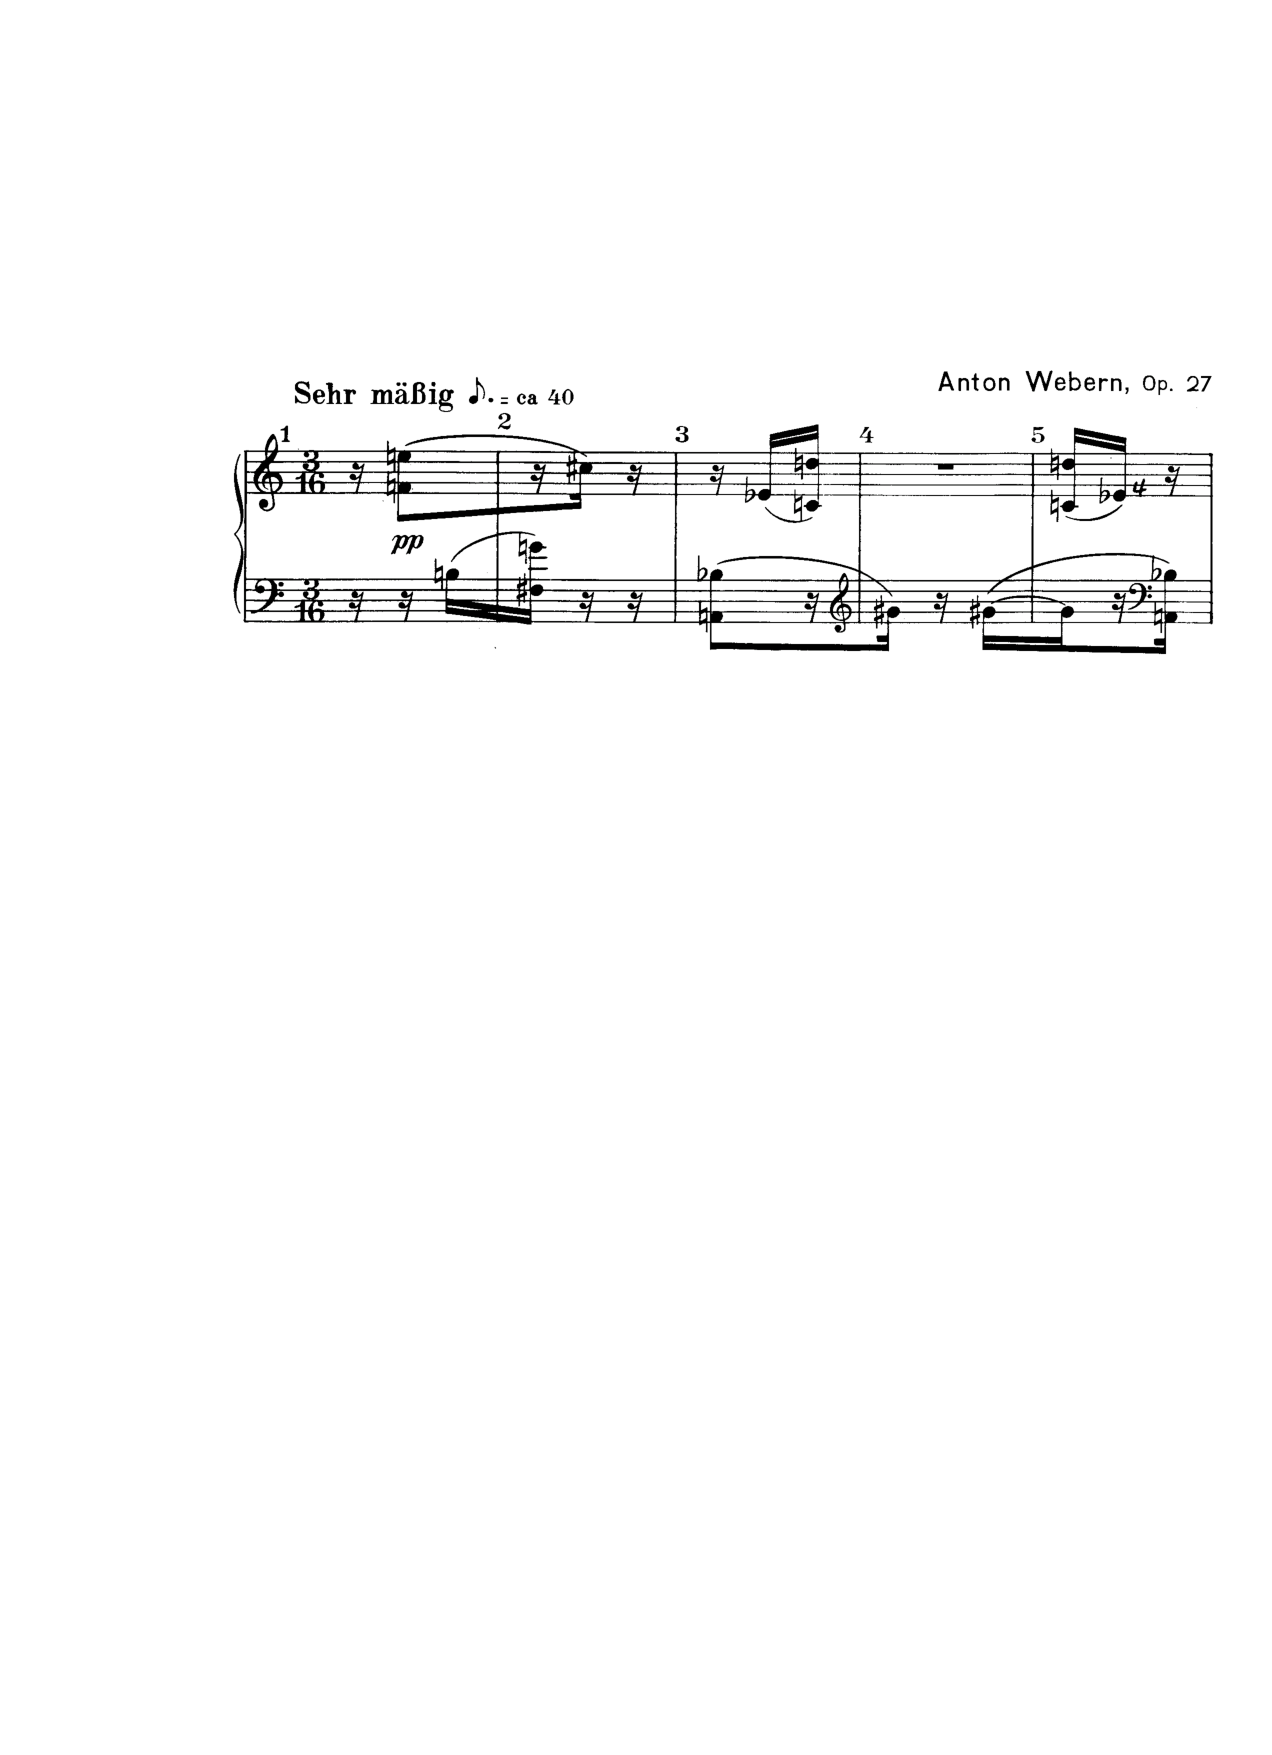
\includegraphics[width=6.5in]{figures/webern1.pdf}
		\caption[Bars 1--7 in Webern's Op.~27]{The initial bars in Webern's Op.~27.}
    	\label{fig:webern-27}
	\end{figure}

    \begin{figure}[htbp]
    	\centering
		\begin{tikzcd}
        	& E \arrow[dr] && G \arrow[dr] && B\flat \arrow[dr] && D \arrow[dr] & \\
        	* \arrow[dr] \arrow[ur] && B \arrow[dr] \arrow[ur] && C\sharp \arrow[dr] \arrow[ur] && E\flat \arrow[dr] \arrow[ur] && G\sharp \\
        	& F \arrow[ur] && F\sharp \arrow[ur] && A \arrow[ur] && C \arrow[ur] &
    	\end{tikzcd}
		\caption[Aggregate Realization of Bars 1--7 in Webern's Op.~27]{An aggregate realization of the initial bars in Webern's Op.~27. At its very first presentation, the total order used to generate the piece cannot be discerned. Moreover, the partial order we are actually able to hear intercalates the total order's two hexachords, a procedure that can be construed as a form of derivation.}
    	\label{fig:webern-aggregate}
	\end{figure}

	\noindent Instead of the aggregate realization in Fig.~\ref{fig:webern-aggregate}, however, we use the fact that we know the basic series is $S = \{ 4, 5, 1, 3, 0, 2, 8, 9, 10, 6, 7, 11 \}$, take the initial bars seen in Fig.~\ref{fig:webern-27}, and rewrite an aggregate realization, call it $D_1$, of them as in Fig.~\ref{fig:webern-aggregate-b}.

	\begin{figure}[htbp]
    	\centering
		\begin{tikzcd}
	    	& [-1em] E \arrow[dr] & [-1em] & [-1em] & [-1em] D \arrow[rd] & [-1em] & [-1em] B\flat \arrow[dr] & [-1em] & [-1em] G \arrow[dr] & [-1em] \\
	    	* \arrow[dr] \arrow[ur] & [-1em] & [-1em] C\sharp \arrow[r] & [-1em] E\flat \arrow[dr] \arrow[ur] & [-1em] & [-1em] G\sharp \arrow[dr] \arrow[ur] & [-1em] & [-1em] * \arrow[dr] \arrow[ur] & [-1em] & [-1em] B \\
	    	& [-1em] F \arrow[ur] & [-1em] & [-1em] & [-1em] C \arrow[ur] & [-1em] & [-1em] A \arrow[ur] & [-1em] & [-1em] F\sharp \arrow[ur] & [-1em]
    	\end{tikzcd}
    	\caption[Another Aggregate Realization of Bars 1--7 in Webern's Op.~27]{We denote the underlying partial order depicted in this aggregate realization by $D_1$.}
    	\label{fig:webern-aggregate-b}
	\end{figure}

	\noindent It is not too far-fetched to assume such an analysis. Whereas Fig.~\ref{fig:webern-aggregate} represented a first-time hearing depiction of bars 1--7, Fig.~\ref{fig:webern-aggregate-b} can be achieved by, say, a performer who realizes the voice-crossing of the series along its reflection axis. Having come to this conclusion, parsing bars 8--10 becomes a bit less daunting. Fig.~\ref{fig:webern-27-b} shows bars 8--10 in Op.~27, and Fig.~\ref{fig:webern-aggregate-c} is a normalized aggregate realization of the passage. By normalized we mean that the series being displayed in the music is $\T_{10}\I(S) = \{ 6, 5, 9, 7, 10, 8, 2, 1, 0, 4, 3, 11 \}$, but instead we set the aggregate realization to $S$, since we will want to take intersections of both partial orders later. $\T_{10}\I(S)$ begins with the right hand in bar 8, moves to the left hand in bar 9, and the very last note (which is not showing) is a high B the right hand again has in bar 11. At this point, our confidence that a series can be heard by the listener is severely damaged. We even start to doubt that the average performer will have obtained, or even cared to obtain, a good grasp on what the series really is.

	\begin{figure}[htbp]
    	\centering
		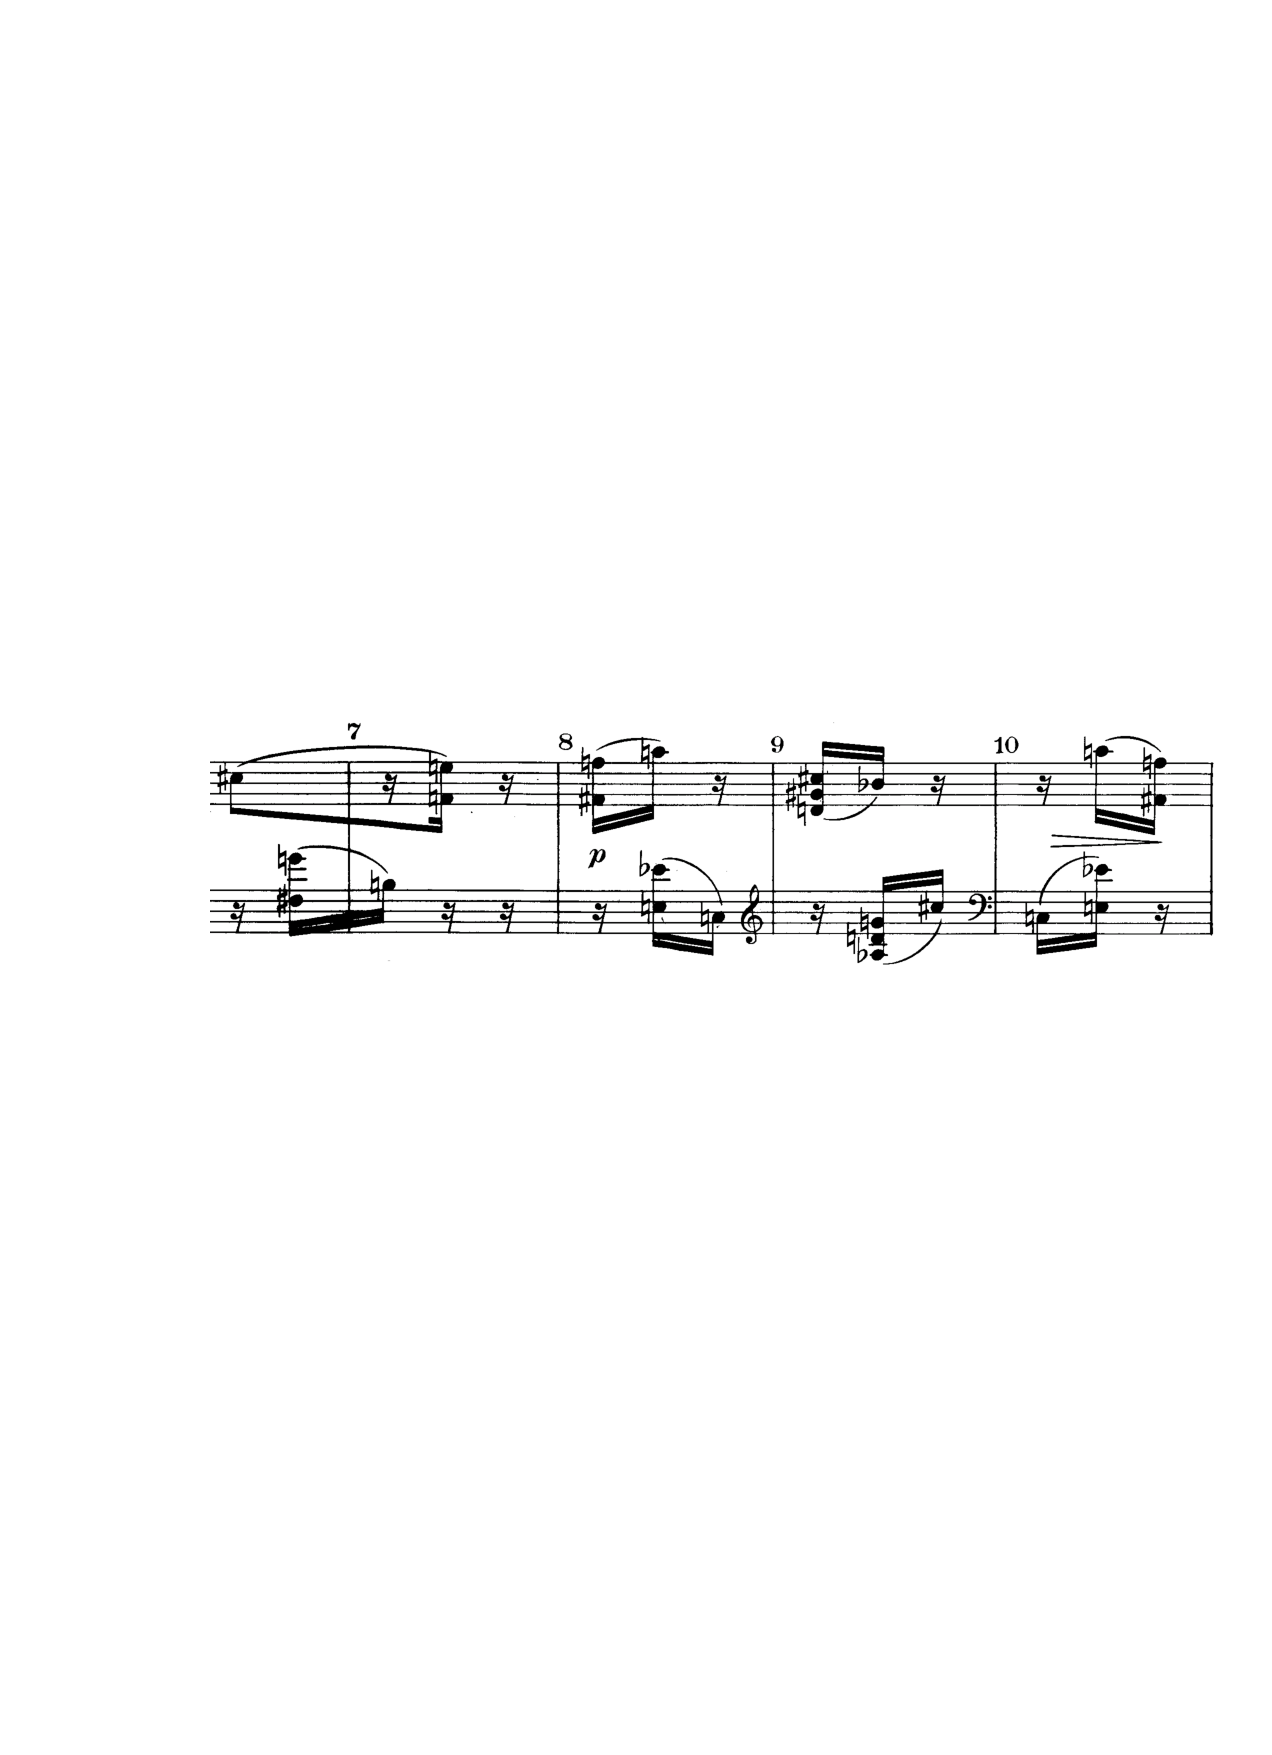
\includegraphics[width=6.5in]{figures/webern2.pdf}
		\caption[Bars 8--10 in Webern's Op.~27]{Bars 8--10 in Webern's Op.~27.}
    	\label{fig:webern-27-b}
	\end{figure}

	\begin{figure}[htbp]
    	\centering
		\begin{tikzcd}
	    	&&& E\flat \arrow[ddr] &&&& \\
	    	& E \arrow[dr] && D \arrow[dr] &&& G \arrow[dr] & \\
	    	* \arrow[ur] \arrow[dr] && C\sharp \arrow[ur] \arrow[dr] \arrow[uur] \arrow[ddr] && A \arrow[r] & B\flat \arrow[ur] \arrow[dr] && B \\
	    	& F \arrow[ur] && C \arrow[ur] &&& F\sharp \arrow[ur] & \\
	    	&&& G\sharp \arrow[uur] &&&&
    	\end{tikzcd}
		\caption[An Aggregate Realization of Bars 8--10 in Webern's Op.~27]{We denote the underlying partial order depicted in this aggregate realization by $D_2$.}
    	\label{fig:webern-aggregate-c}
	\end{figure}

	\noindent The next excerpt we analyze in the first movement is the last one we need in order to infer what series Webern used for the piece. The musical passage, taken from bars 19--23, is given in Fig.~\ref{fig:webern-27-c}, and an aggregate realization is displayed in Fig.~\ref{fig:webern-aggregate-d}. We again normalize it with respect to $S$. This time, the series we are looking for in the excerpt is $\T_3\I(S) = \{ 11, 10, 2, 0, 3, 1, 7, 6, 5, 9, 8, 4 \}$, and again it has a very convoluted presentation, floating around in register, and freely changing hands. We come to the realization that, without the score, it is unlikely that a listener, even a very educated one, will be able to discern the composer's main generative material in one hearing. That well-versed listener might not be able to discern it in the hundredth hearing, we even suspect. We shall conclude the analysis before coming back to this discussion, however.

	\begin{figure}[htbp]
    	\centering
		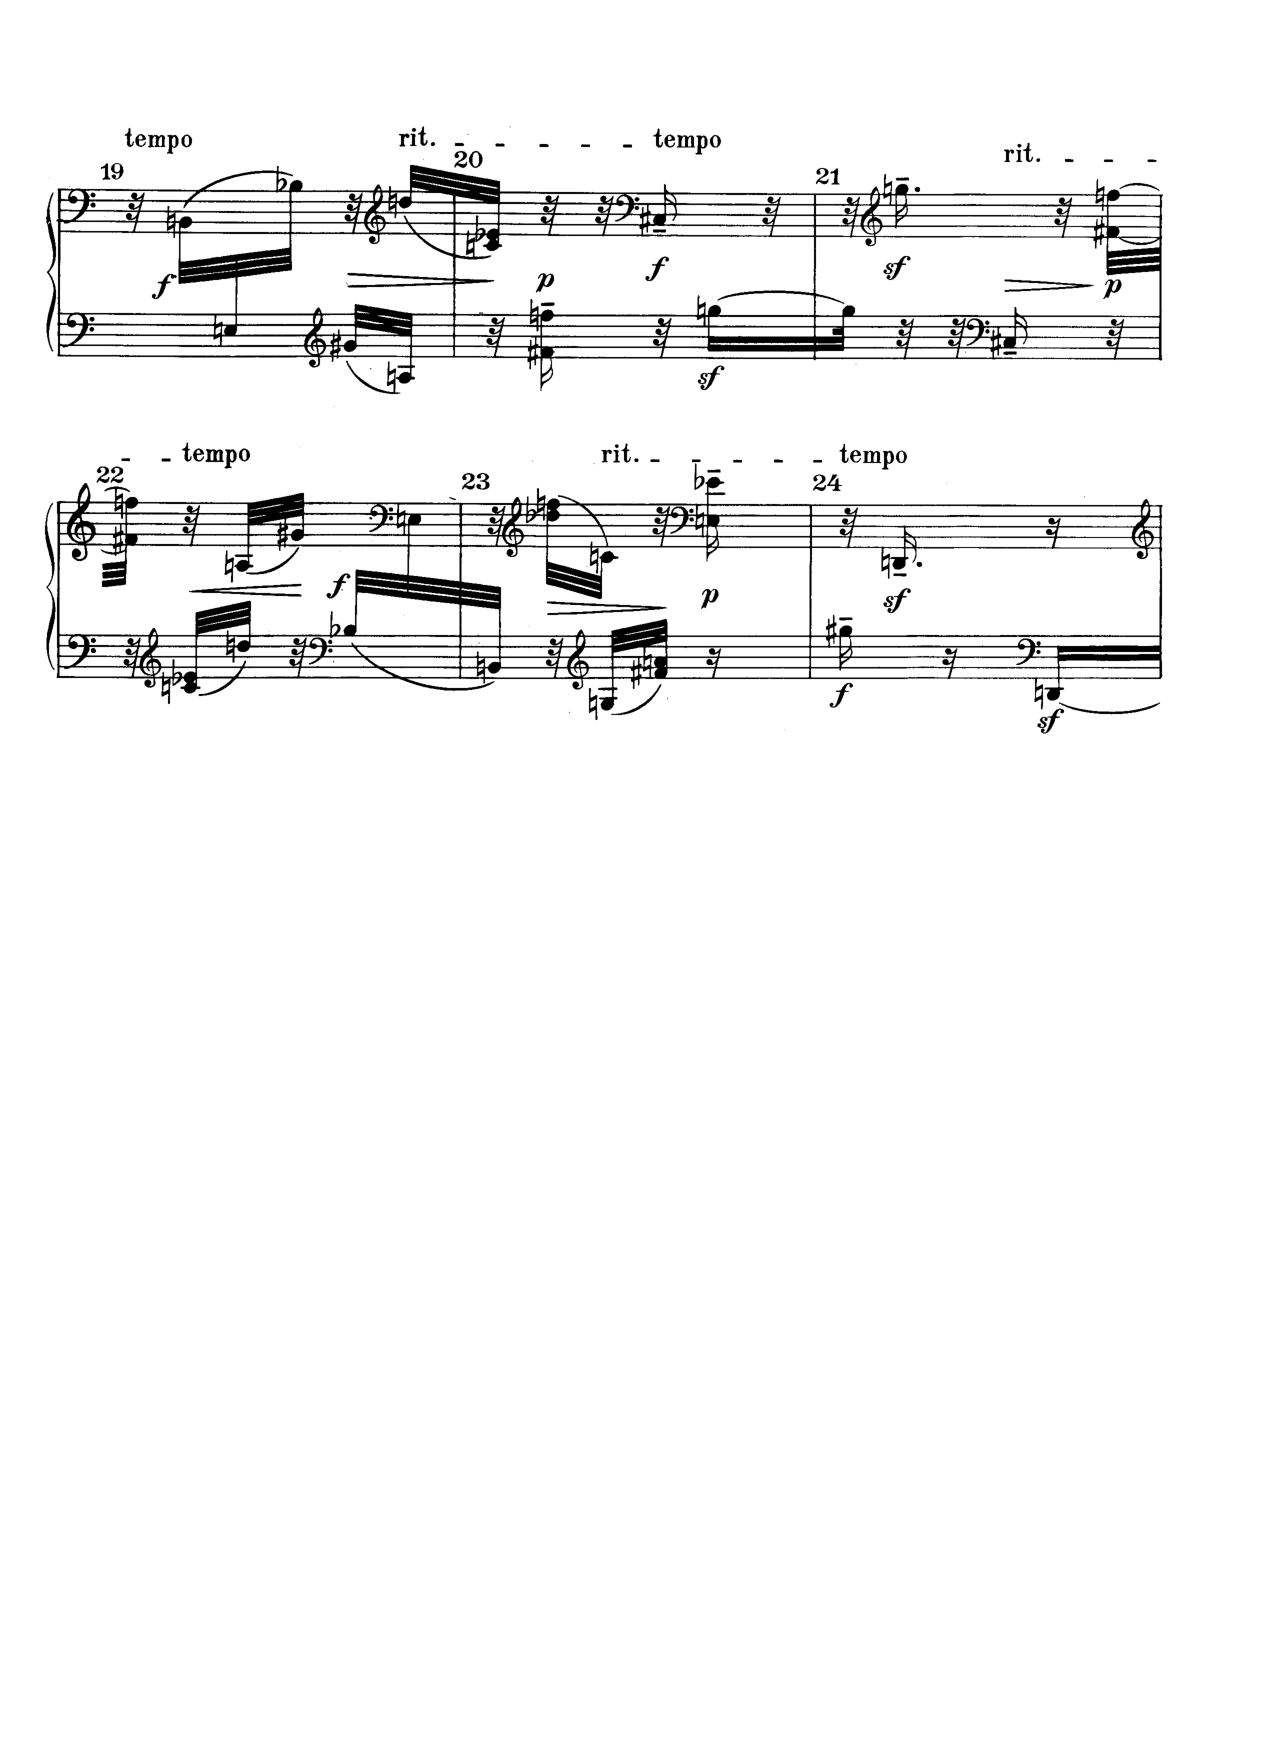
\includegraphics[width=6.5in]{figures/webern3.pdf}
		\caption[Bars 19--23 in Webern's Op.~27]{Bars 19--23 in Webern's Op.~27.}
    	\label{fig:webern-27-c}
	\end{figure}

	\begin{figure}[htbp]
    	\centering
		\begin{tikzcd}
	    	& [-1em] & [-1em] & [-1em] E\flat \arrow[dr] & [-1em] & [-1em] & [-1em] B\flat \arrow[dr] & [-1em] & [-1em] & [-1em] \\
	    	E \arrow[r] & [-1em] F \arrow[r] & [-1em] C\sharp \arrow[ur] \arrow[dr] & [-1em] & [-1em] D \arrow[r] & [-1em] G\sharp \arrow[ur] \arrow[dr] & [-1em] & [-1em] F\sharp \arrow[r] & [-1em] G \arrow[r] & [-1em] B \\
	    	& [-1em] & [-1em] & [-1em] C \arrow[ur] & [-1em] & [-1em] & [-1em] A \arrow[ur] & [-1em] & [-1em] & [-1em]
    	\end{tikzcd}
		\caption[An Aggregate Realization of Bars 19--23 in Webern's Op.~27]{We denote the underlying partial order depicted in this aggregate realization by $D_3$.}
    	\label{fig:webern-aggregate-d}
	\end{figure}

	\noindent The last step in figuring out Webern's total order, according to our theoretical assumptions so far, is to take intersections of the partial orders depicted above with aggregate realizations. Assuming one could actually hear the presentation of the series without being victimized by any of the numerous pitfalls represented by all the registral displacements in the piece, and furthermore assuming one could freely invert and transpose twelve ordered and different pitch classes in their heads almost instantly, one would possibly arrive with the intersection $D_1 \cap D_2$ at measure 10. An aggregate realization of the intersection is shown in Fig.~\ref{fig:webern-aggregate-e}. One would still be puzzled, however, since there are still three incomparabilities that prevent one from comprehending the underlying series.

	\begin{figure}[htbp]
    	\centering
		\begin{tikzcd}
	    	& [-1em] E \arrow[dr] & [-1em] & [-1em] & [-1em] D \arrow[dr] & [-1em] & [-1em] & [-1em] & [-1em] G \arrow[dr] & [-1em] \\
	    	* \arrow[ur] \arrow[dr] & [-1em] & [-1em] C\sharp \arrow[r] & [-1em] E\flat \arrow[ur] \arrow[dr] & [-1em] & [-1em] G\sharp \arrow[r] & [-1em] A \arrow[r] & [-1em] B\flat \arrow[ur] \arrow[dr] & [-1em] & [-1em] B \\
	    	& [-1em] F \arrow[ur] & [-1em] & [-1em] & [-1em] C \arrow[ur] & [-1em] & [-1em] & [-1em] & [-1em] F\sharp \arrow[ur] & [-1em] \\
    	\end{tikzcd}
		\caption[Intersecting Bars 1--7 with Bars 8--10 in Webern's Op.~27]{The intersection $D_1 \cup D_2$.}
    	\label{fig:webern-aggregate-e}
	\end{figure}

	\noindent The next two pictures depict aggregate realizations for the intersections $D_1 \cap D_3$ and $D_2 \cap D_3$. Having reached measure 23, we are finally in a position to obtain Webern's series. Both intersections, however, still carry incomparabilities, so we will only be able to achieve our goal by taking the intersection of all three aggregate realizations.

	\begin{figure}[htbp]
    	\centering
		\begin{tikzcd}
	    	& [-1em] & [-1em] & [-1em] & [-1em] & [-1em] & [-1em] & [-1em] B\flat \arrow[dr] & [-1em] & [-1em] & [-1em] \\
	    	E \arrow[r] & [-1em] F \arrow[r] & [-1em] C\sharp \arrow[r] & [-1em] E\flat \arrow[r] & [-1em] C \arrow[r] & [-1em] D \arrow[r] & [-1em] G\sharp \arrow[ur] \arrow[dr] & [-1em] & [-1em] F\sharp \arrow[r] & [-1em] G \arrow[r] & [-1em] B \\
	    	& [-1em] & [-1em] & [-1em] & [-1em] & [-1em] & [-1em] & [-1em] A \arrow[ur] & [-1em] & [-1em] & [-1em]
    	\end{tikzcd}
		\caption[Intersecting Bars 1--7 with Bars 19--23 in Webern's Op.~27]{The intersection $D_1 \cup D_3$.}
    	\label{fig:webern-aggregate-f}
	\end{figure}

	\begin{figure}[htbp]
    	\centering
		\begin{tikzcd}
	    	& [-1em] & [-1em] & [-1em] E\flat \arrow[dr] & [-1em] & [-1em] & [-1em] & [-1em] & [-1em] & [-1em] & [-1em] \\
	    	E \arrow[r] & [-1em] F \arrow[r] & [-1em] C\sharp \arrow[ur] \arrow[dr] && [-1em] D \arrow[r] & [-1em] G\sharp \arrow[r] & [-1em] A \arrow[r] & [-1em] B\flat \arrow[r] & [-1em] F\sharp \arrow[r] & [-1em] G \arrow[r] & [-1em] B \\
	    	& [-1em] & [-1em] & [-1em] C \arrow[ur] & [-1em] & [-1em] & [-1em] & [-1em] & [-1em] & [-1em] & [-1em]
    	\end{tikzcd}
		\caption[Intersecting Bars 8--10 with Bars 19--23 in Webern's Op.~27]{The intersection $D_2 \cup D_3$.}
    	\label{fig:webern-aggregate-g}
	\end{figure}

	\noindent It is with bitter-sweet joy that we finally declare victory in Fig.~\ref{fig:webern-aggregate-h}, as we know we would not stand a chance relying on hearing alone.

	\begin{figure}[htbp]
    	\centering
		\begin{tikzcd}
	    	E \arrow[r] & [-1em] F \arrow[r] & [-1em] C\sharp \arrow[r] & [-1em] E\flat \arrow[r] & [-1em] C \arrow[r] & [-1em] D \arrow[r] & [-1em] G\sharp \arrow[r] & [-1em] A \arrow[r] & [-1em] B\flat \arrow[r] & [-1em] F\sharp \arrow[r] & [-1em] G \arrow[r] & [-1em] B
    	\end{tikzcd}
		\caption[The intersection of Bars 1--7, 8--10, and 19--23 in Webern's Op.~27]{The intersection $D_1 \cup D_2 \cup D_3$.}
    	\label{fig:webern-aggregate-h}
	\end{figure}

\end{example}

There is much to be said about Ex.~\ref{starr-webern-example}, particularly in what regards the aural perception of the composer's constructs. There is even more to be said if we take into consideration the fact that, as the twentieth-century unraveled, it became in many cases increasingly more difficult to establish how a piece of music was constructed with the presence of the score alone, much less simply by aural inference. It becomes less straightforward to determine the role of the listener in these cases, especially whenever one insists that the listener should be able to aurally infer \emph{every} construct in a musical composition. We argue here that, as composers differentiate themselves from common practice, compositional technique becomes more subjective, and often indiscernible in the musical discourse. That does not mean, however, that musical fruition should be hindered in any sense, or that the composer's channel of communication with the listener has been narrowed in any way. It is simply the case that, even when not every single part of a structure is fathomed, we are still able to experience the structure itself. We do not need a blueprint to live in a house, we do not need a wrench to drive a car, and we certainly do not begin to understand the intricacies of the very universe in which we exist. And we do exist nonetheless.

The role of the analyst, on the other hand, also becomes more difficult to define. Whenever the structure of a piece of music becomes impossible to follow from its score alone, a theorist must reconsider the weight of musicological work in the analysis of such repertoire. In other words, it may very well be impossible to analyze a composition without resorting to the composer, or to a musicological study thereof. That is especially the case with algorithmic composition, which is a major avenue to which we shall apply our main object of study. Analyzing an algorithmically generated piece of music without prior knowledge of the algorithm itself can only go as far as devising hearing strategies for the piece, as well as conjecturing what the algorithm might have been. It may be of substantial value, it may even carry more value than an analysis of the algorithm itself. And, just like with any piece of software, understanding the code is not a prerequisite to using said software, much less to determining whether it fulfills its purpose, or whether it is a good piece of software or not. However, if one intends to determine precisely how a piece of music was \emph{constructed}, then knowledge of its blueprint becomes essential. And that determination is often of primary interest to composers.

The compositional techniques we are about to define and generalize in this study are notoriously of structural relevance. It does not mean that they cannot be aurally discerned, and in fact many authors devote considerable time devising hearing strategies for them, particularly when they are used to structure pitch. Nevertheless, our approach here will be restricted to the intrinsic qualities of these techniques, and we shall not pursue their aural perception in depth, simply because there may not be any intention from the composer's part for them to be heard at all. A familiar example might be the music of Stravinsky. Upon analyzing his use of rotational arrays, it becomes clear that the composer uses them as a generative techniques, rather than as a foreground musical entities. Analyzing such pieces often resort to techniques that have no connection whatsoever to any sort of hearing strategy, like Forte's employment of K and Kh set complexes, which yield a nexus set that ultimately cannot be heard. We aggravate this discussion with the idea that, more often than not, we shall employ the techniques we are about to present to dimensions other than pitch, and in particular to algorithmically determining spectral components and timbre. In this sense, their outcomes become textural elements of a composition, but still well within the canon of tasks a composer needs to exercise in the craft of a piece.

Whereas aggregate realizations correspond to a totally ordered sequence of disjoint subsets of the free aggregate, a \emph{columnar (aggregate) realization} is, on the other hand, a set of disjoint row segments where, even though the internal order of each segment is total, all segments are pairwise incomparable. In addition, we require that a columnar realization contain the free aggregate as a subset, so that we get all pitch classes belonging to a given base in every column. This is essentially a combination matrix in twelve-tone theory.

\begin{example}
    \cite[201, 210]{Starr1984}
    The intersection of the set of all aggregate realizations with the set of all columnar realizations contains the set of all total orders (and thus all row segments), as well as the free aggregate. A total order is trivially an aggregate realization, and it is trivially a columnar realization. Any total order contains the free aggregate per our requirements.
\end{example}

%--------------------------------------------------------------------------
\subsection{Row Segments}

The concept of a \emph{row segment}, which is fairly straightforward in twelve-tone theory, has an analogue here in the sense that we define it as a pitch-class relation that is reflexive, transitive, and antisymmetric. We impose the additional requirement that some subset of its order constraints also satisfy trichotomy. Arguably more important is the concept of an \emph{embedded segment}. For any partial order that covers some row segment, we say that segment is an embedded segment of the partial order. By transitivity of covering, any other partial order covering the former partial order will have the aforementioned row segment embedded in it, including naturally any total order in its total order class. In this sense, a partial order may be seen as the union (possibly the extension thereof) of its various embedded segments:

\begin{example}
    \label{starr-common-tones}
    \cite[200]{Starr1984}
    Consider two total orders $X = \{ 0, 1, 7, 2, 10, 9, 11, 4, 8, 5, 3, 6 \}$ and $Y = \{ 1, 2, 8, 3, 11, 10, 0, 5, 9, 6, 4, 7 \}$ where, in particular, $Y = \T_1(X)$. Seen as total orders, one can take the intersection $X \cap Y$, then prune it. This process yields a graph whose longest row segments are $\{ 1, 2, 10, 9, 4 \}$, $\{ 1, 2, 10, 5, 6 \}$, $\{ 1, 2, 11, 5, 6 \}$, $\{ 1, 2, 8, 5, 6 \}$, and $\{ 1, 2, 8, 3, 6 \}$. These row segments are, in turn, the longest that are embedded segments of both $X$ and $Y$.
\end{example}

It is interesting to point out that the procedure described in Ex.~\ref{starr-common-tones} is in fact an algorithm to find common tones under transposition, and can be extended to any other pitch-class operation. This is a much needed addition to a the well-known technique of \emph{counting} common tones.

\begin{theorem}
	\label{rahn-common-tone}
	\cite[10]{Rahn1975}
	The number of common tones between a set $S$ and some transposition of itself is given by
	\begin{equation}
		|S \cap \T_n(S)| = |\{x - y = n : x, y \in S\}| \enspace.
	\end{equation}
	The number of common tones between a set $S$ and some inversion of itself is given by
	\begin{equation}
		|S \cap \T_n\I(S)| = 2 \cdot |\{x + y = n : x, y \in S\}| + |\{a \in S : 2a = n\}| \enspace.
	\end{equation}
	Moreover, the cardinality of the set $\{a \in S : 2a = n\}$ is at most 2.
	\begin{proof}
		We must count the occurrences of pairs of pitch classes that are interchanged by the operation at hand and double them, for if $x$ maps onto $y$ under some $\T_n\I$, then certainly $y$ maps onto $x$ under the same operation, given that every inversion operation has order two. In addition to that, we must account for the occurrences of pitch classes that may map onto themselves under the aforementioned operation. For any pair $a \ne b \in S$, it follows $a$ and $b$ are exchanged by some operation $\T_n\I$ whenever both $\T_n\I(a) = b$ and $\T_n\I(b) = a$ hold. Since $\T_n\I(a) = -a + n$, and similarly $\T_n\I(b) = -b + n$, if the pair is exchanged, then we must have $-a + n = b$ and $-b + n = a$ both true. Adding the last two expressions and yields $a + b = n$, which is the first set in the right-hand side of the formula. As discussed above, the cardinality of this set must be doubled. We have for any $a$ that $\T_n\I(a) = a + n$, hence $a = \T_n\I(a) \iff a = -a + n$, that is, whenever $2a = n$. That is the second set in the formula. Finally, for any pair $(a, n)$ such that $a = \T_n\I(a)$, we also have $a + 6 = -(a + 6) + n \iff 2a = n$, so that by the above it follows $a + 6 = \T_n\I(a + 6)$. Thus the set $\{a \in S : 2a = n\}$ has cardinality at most 2, proving the last assertion.
	\end{proof}
\end{theorem}

\begin{example}
    \label{rahn-example}
    \cite[11]{Rahn1975}
    Write $S = \{ 0, 1, 4, 5, 8, 9 \}$ and consider some inversion operation. An application of Th.~\ref{rahn-common-tone} yields the table below.
    \begin{table}[htbp]
    \caption[Rahn's Common Tones Under Inversion]{Common tones under inversion between $S = \{ 0, 1, 4, 5, 8, 9 \}$ and itself.}
    \centering
    \vspace{12pt}
    \begin{tabular}{ c | *{12}{c} }
        \hline\\
        $n$ & 0 & 1 & 2 & 3 & 4 & 5 & 6 & 7 & 8 & 9 & 10 & 11 \\\\
        $2 \cdot |\{x + y = n : x, y \in S\}|$ & 2 & 6 & 2 & 0 & 2 & 6 & 2 & 0 & 2 & 6 & 2 & 0 \\\\
        $|\{a \in S : 2a = n\}|$ & 1 & 0 & 1 & 0 & 1 & 0 & 1 & 0 & 1 & 0 & 1 & 0 \\\\
        \hline\\
        Total & 3 & 6 & 3 & 0 & 3 & 6 & 3 & 0 & 3 & 6 & 3 & 0 \\\\
        \hline
    \end{tabular}
    \end{table}
\end{example}

In practice, however, many composers choose to compute common tones by writing down an entire matrix. This procedure has the advantage of, not only giving all indices of transposition under which a set shares common tones with itself or other set, but it is also possible to determine whether these common tones will preserve their ordering after the transform by examining the matrices' diagonals.

\begin{example}
	\cite[49]{Morris1987}
    \label{morris-common-tones}
    Let $X$ be an $n$-tone row seen as a column vector, and consider the $n \times n$ matrix $A = [X, \cdots, X]$. In particular, the matrix $B = A - A^T$ will have a main diagonal of zeros, which indicates that $X$ shares with itself $n$ common tones under $T_0$. If there are $k$ threes in the matrix, then $X$ will share with itself $k$ tones under $T_3$. There is no requirement that we compare a row with itself. If, for instance, $A$ is given as above, and $\bar{A}$ is the matrix for the row $\bar{X}$, then counting the number $k$ of, say, threes in $B = A - \bar{A}^T$, will mean in turn that $X$ and $\T_3(\bar{X})$ share $k$ tones under $\T_3$. Naturally, the main diagonal of $B$ will not comprise only zeros if $A \ne \bar{A}$. To find common tones under inversion, we let $B = A + A^T$ and, similarly, $\M$ and $\M \circ \I$ become $B = A - \M(A)^T$ and $B = A + \M(A)^T$. Finally, if the indices we are counting are disposed in any of the matrix's diagonals, then they will preserve ordering after the transform, thus becoming embedded segments; if, in addition, they are adjacent, then they will in fact be row segments shared by $X$ and the transform of $\bar{X}$.
\end{example}

The matrix for finding common tones under transposition that is described in Ex.~\ref{morris-common-tones} has the interesting property that it becomes a symmetric matrix when $A = \bar{A}$ and we take its elements as interval classes. This reflects the fact that, if $X$ shares $k$ tones with $T_i(X)$, then surely $T_i(X)$ will share exactly $k$ tones with $T_{12 - i}(X)$. If $i$ is an interval class, then $i = 12 - i$, showing why the matrix will be symmetric. The matrix of common tones under inversion is always symmetric, regardless we take its elements as interval classes. For multiplicative operations, however, we will often lack multiplicative inverses in twelve tones. For $p$-TET systems where $p$ is prime, we do get symmetric matrices for multiplicative operations as well, but those will sometimes require a proper definition of multiplicative interval classes.

The importance of the procedure described in Ex.~\ref{starr-common-tones} is due to the fact that the technique in Ex.~\ref{morris-common-tones} can only go as far as counting the number of common tones, whereas the former procedure can actually tell us \emph{what} these common tones are in a more straightforward manner. In addition, it can be very computationally effective if we write the rows we wish to compare as binary square matrices describing their order constraints. Taking then their intersection is easy, since we can rely on binary operations for this type of matrix. Pruning, if we wish to express the result as a graph, is also fast and simple. That being said, neither the above techniques addresses one of our primary concerns regarding derivation: given a set of order numbers and a transformation, what series are capable of producing transforms of \emph{themselves} when pulled from those order numbers. This is in essence the exact opposite of what we have demonstrated above, where we depart from a series and attempt to understand its embedded segments. And it is arguably not a coincidence, as much of the twelve-tone theory devised since Forte has a strong analytical bias. What we are mainly interested, however, is in how these techniques fit onto the compositional scheme of things. And for that, having a two-way street where, on one hand we understand raw compositional materials and, on the other, we formulate them, is crucial. Moreover, as we attempt to construe orderedness as a generative procedure in all generality, it becomes imperative that we break our ties with purely analytical music theory and begin to delve into the mathematics of these general constructs. As the example below suggests, mathematics can greatly simplify the way we approach certain concepts and, depending on the task at hand, may even be decisive in determining whether it is feasible or not to pursue certain compositional avenues. For algorithmic composition, in particular, having a firm theoretical understanding of some generative procedure can greatly simplify the composer's algorithm, as well as make it more efficient.

\begin{example}
	We can demonstrate \ref{rahn-example}, and also the omitted proof of \ref{rahn-common-tone} under transposition in a much simpler way with a little bit of abstract algebra by observing the cycle decomposition of each operation at hand. If $n = 3$, then we have
	\begin{equation}
		\T_3\I = (0 \; 3) (1 \; 2) (4 \; 11) (5 \; 10) (6 \; 9) (7 \; 8) \enspace.
	\end{equation}
	Hence, under $\T_3\I$, every pitch-class in $S = \{ 0, 1, 4, 5, 8, 9 \}$ maps to the complement of $S$. If the operation is, for instance, $\T_9$, then since
	\begin{equation}
		\T_9 = (0 \; 9 \; 6 \; 3) (1 \; 10 \; 7 \; 4) (2 \; 11 \; 8 \; 5) \enspace,
	\end{equation}
	we get straightforwardly that $S = \{ 0, 1, 4, 5, 8, 9 \}$ shares three common tones with $\T_9(S)$, namely $0 \mapsto 9$, $4 \mapsto 1$, and $8 \mapsto 5$.
\end{example}

In a completely analogous manner to the principle of pulling row segments from a series, and in the interest of building two-way roads, we can most certainly concatenate row segments in order to formulate a new series. 

\begin{example}
    \cite[200]{Starr1984}
    Let $X = \{ 0, 1, 2 \}$ and $Y = \{ 3, 4, 5 \}$ be row segments. We actually require that $X \cap Y = \emptyset$ when seeing $X$ and $Y$ as partial orders. The concatenation $X | Y$ will then be the partial order:
    \begin{equation}
        X \cup Y \cup \{ \{ a, b \} : a \in X, b \in Y \} \enspace.
    \end{equation}
    It follows immediately that both $X$ and $Y$ are embedded row segments of $X | Y$. Note that our use of concatenation here is sequential, that is, the entire row segment $X$ precedes the entire row segment $Y$ in $X | Y$. In other words, we do not allow intercalation of segments when concatenating.
\end{example}

%--------------------------------------------------------------------------
\section{A Survey of Derivation Techniques}

In this section we devote our attention to expanding the idea first presented in Ex.~\ref{ex:derivation}. In it, we devise a type of derivation in which the series being displayed vertically is unrelated to the series being derived horizontally, except for the fact that both share a row segment when we retrograde one of the rows. The construction is part of a more general procedure, in which we always match a row with a retrograded transform of itself. In the particular case of Ex.~\ref{ex:derivation}, the transform, say $F$, was $\T_0$ for simplicity, but arbitrary pitch-class operations may be used. Denote the given series by $S$, and define similarly the derived row as $V = V_1 | V_2$, that is, $V$ is a concatenation of two row segments. The only requirement is that $V_1$, the segment we choose to single out, remains invariant under $F$, which will force $V_2$ to also be invariant under $F$. In Ex.~\ref{ex:derivation} this requirement is satisfied trivially. The aforementioned procedure is given schematically in Table~\ref{derivation-retrograde}.

\begin{table}[htbp]
    \caption[Derivation Involving the Retrograde and an Arbitrary Operation]{Schematics of a derivation procedure involving the retrograde and an arbitrary operation $F$.}
    \label{derivation-retrograde}
    \centering
    \vspace{12pt}
    \begin{tabular}{c|cc}
        \hline\\
        & $S$ & $\R \circ F(S)$\\\\
        \hline\\
        $V$ & $V_1$ & $V_2$ \\\\
        $\R \circ F(V)$ & $\R \circ F(V_2)$ & $\R \circ F(V_1)$ \\\\
        \hline
    \end{tabular}
\end{table}

\begin{example}
    \label{ex:derivation-ordered}
    In this example, we illustrate a derivation procedure similar to that in Ex.~\ref{ex:derivation} where the operation $F$ is not trivial. We again take the row in Berg's \emph{Lulu}, $S = \{ 10, 2, 3, 0, 5, 7, 4, 6, 9, 8, 1, 11 \}$, and consider the segment $\vec{s} = [10 \; 0 \; 5 \; 7]^T$ as a column vector. Now let $A^T = [\;\vec{s} \; | \; \vec{s} \; | \; \vec{s} \; | \; \vec{s}\;]$ be the square matrix whose every column is equal to $\vec{s}$. Then
	\begin{equation}
    	A + A^T = \begin{bmatrix}
    		2 & 10 & 3 & 5 \\
        	10 & 0 & 5 & 7 \\
        	3 & 5 & 10 & 0 \\
        	5 & 7 & 0 & 2
        \end{bmatrix} \pmod{12} \enspace.
	\end{equation}
	\noindent In particular, we see that the row segment $\{ 10, 0, 5, 7 \}$ is invariant under $\R\T_5\I$, since we get a main diagonal of fives when we mirror the matrix above vertically. Thus, by matching $S$ with $\R\T_5\I(S)$, we may get the row segment $\{ 10, 0, 5, 7 \}$ in the derived row $V$ itself, rather than in its retrograde, as was the case in Ex.~\ref{ex:derivation}. Setting it to $V_2$, say, yields $V = \{ 2, 3, 4, 6, 9, 8, 1, 11, 10, 0, 5, 7 \}$, so we get the combination matrix below.
	\begin{equation}
    	\left[
    	\begin{array}{cccccccccccc|cccccccccccc}
        	. & 2 & 3 & . & . & . & 4 & 6 & 9 & 8 & 1 & 11 & . & . & . & . & . & . & 10 & 0 & 5 & . & . & 7 \\
        	10 & . & . & 0 & 5 & 7 & . & . & . & . & . & . & 6 & 4 & 9 & 8 & 11 & 1 & . & . & . & 2 & 3 & .
    	\end{array}
    	\right] \enspace.
	\end{equation}
\end{example}

It is usually the case in this type of derivation that, unlike Ex.~\ref{ex:derivation-ordered}, the invariance of $V$ under $F$, or under $\R \circ F$ for that matter, does not preserve any ordering.

\begin{example}
    \cite[212]{Starr1984}
    Let $S = \{ 0, 1, 7, 2, 10, 9, 11, 4, 8, 5, 3, 6 \}$ and consider the operation
    \begin{equation}
        \T_2\I = (0 \; 2) (3 \; 11) (4 \; 10) (5 \; 9) (6 \; 8) \enspace.
    \end{equation}
    Upon inspection of the cycles of $\T_2\I$, we see that the segment $\{ 0, 1, 7, 2 \}$ is invariant under it. If we consider a combination matrix involving $\R\T_2\I$, however, then we shall not obtain the same ordered result as in Ex.~\ref{ex:derivation-ordered}, since both $(1)$ and $(7)$ are fixed points. The same would happen to any $\T_k\I$ where $k$ is even. In particular, this shows that, in order to obtain the same ordered row segment in both columns of the combination matrix, $F$ cannot be trivial.
	\begin{equation}
    	\left[
    	\begin{array}{cccccccccccc|cccccccccccc}
        	0 & . & . & 1 & . & 7 & . & . & . & 2 & . & . & 10 & 9 & . & 11 & 4 & 8 & . & 5 & . & 3 & 6 & . \\
        	. & 8 & 11 & . & 9 & . & 6 & 10 & 3 & . & 5 & 4 & . & . & 0 & . & . & . & 7 & . & 1 & . & . & 2
    	\end{array}
    	\right] \enspace.
	\end{equation}
\end{example}

As a consequence of $F$ and the retrograde operation, combination matrices of this type feature two columns that are upside down $F$-mirrors of each other. In line with our theoretical remarks so far, more can be said about such combination matrices.

\begin{proposition}
    \cite[211, 214]{Starr1984}
    Consider a 2-row combination matrix $C$ where a row is derived via the retrograde and some operation $F$. Denote the derived row by $V = V_1 | V_2$. Then the first column is the partial order $C_1 = V_1 \cup \R \circ \F(V_2)$, and similarly the second column is the partial order $C_2 = V_2 \cup \R \circ \F(V_1)$, such that $C_2 = \R \circ F(C_1)$. If $D$ is a partial order that covers $C_1$, then $\R \circ F(D)$ will cover $C_2$, and if $D$ is in the total order class of $C_1$, that is, $D$ is a row that can be linearized from $C_1$, then $\R \circ F(D)$ is in the total order class of $C_2$. Finally, 2-row derivations of this type exist for arbitrary rows. The number of such combination matrices for any given row depends on the invariances of the chosen partition of $V$. 
\end{proposition}

It is not clear from the literature, however, how many 2-row combination matrices involving $\R$ we can get for an arbitrary row \emph{exactly}. We shall investigate what this number is in the present study.

%--------------------------------------------------------------------------
\subsection{Folded Derivation}

A related technique involving greater than 2-row counterpoint is achieved by \emph{folding} a derivation matrix. The process is equivalent to first constructing a matrix of hexachordal combinatoriality in the traditional sense, that is, where hexachords are seen as tropes rather than as row segments, then deriving rows from this matrix using the techniques above. Let $S$ be a row whose first hexachord is invariant under the operation $G$. Consider a row $V = V_1 | V_2$ and an operation $F$ such that $S$ is in the total order order class of $V_1 \cup \R \circ \F(V_2)$. Then putting $S$ in counterpoint with $G(S)$, as well as deriving $V$ from $S | \R\circ F(S)$ yields the schematic representation in Table~\ref{derivation-folded}:

\begin{table}[htbp]
    \caption[Folded Derivation Involving the Retrograde]{Schematics of a folded derivation procedure involving the retrograde.}
    \label{derivation-folded}
    \centering
    \vspace{12pt}
    \begin{tabular}{c|cc}
        \hline\\
        & $S$ & $\R \circ F(S)$\\\\
        \hline\\
        $V$ & $V_1$ & $V_2$ \\\\
        $\R \circ F(V)$ & $\R \circ F(V_2)$ & $\R \circ F(V_1)$ \\\\
        $\R \circ GF(V)$ & $\R \circ GF(V_2)$ & $\R \circ GF(V_1)$ \\\\
        $G(V)$ & $G(V_1)$ & $G(V_2)$ \\\\
        \hline\\
        & $G(S)$ & $\R \circ GF(S) = \R \circ FG(S)$ \\\\
        \hline
    \end{tabular}
\end{table}

It is argued without proof in \cite[215]{Starr1984} that, for a derivation procedure such as the one in Table~\ref{derivation-folded}, the folded derivation has to vertically satisfy $G$, while satisfying $F$ horizontally. Thus $F$ and $G$ would have to commute in this case. The caveat that the operation chosen for the hexachordal combinatoriality part must commute with the operation chosen for the derivation part still needs to be confirmed, however, as other derivation matrices that have similar constraints do not require commutativity. Ex.~\ref{derivation-folded} shows a musical application of folded derivations.

\begin{example}
    \cite[215]{Starr1984}
    \label{ex:derivation-folded}
    Let $S = \{ 0, 1, 11, 3, 8, 10, 4, 9, 7, 6, 2, 5 \}$ and consider the operation $\T_6$:
    \begin{equation}
        \T_6 = (0 \; 6) (1 \; 7) (2 \; 8) (3 \; 9) (4 \; 10) (5 \; 11) \enspace.
    \end{equation}
    Let $V_1 = \{ 1, 3, 8, 9, 7, 2 \}$. In particular, since the unordered set $V_1$ is $T_6$-invariant, we get $V_2 = \{ 11, 0, 10, 4, 5, 6 \}$ and the following combination matrix:
    \begin{equation}
        \left[
        \begin{array}{cccccccccccc|cccccccccccc}
            & 1 && 3 & 8 &&& 9 & 7 && 2 && 11 && 0 &&& 10 & 4 &&& 5 && 6 \\
            0 && 11 &&& 10 & 4 &&& 6 && 5 && 8 && 1 & 3 &&& 2 & 9 && 7 &  
        \end{array}
        \right] \enspace.
    \end{equation}
    Consider further the operation $\T_5\I$:
    \begin{equation}
        \T_5\I = (0 \; 5) (1 \; 4) (2 \; 3) (6 \; 11) (7 \; 10) (8 \; 9) \enspace.
    \end{equation}
    Then $S_1 = \{ 0, 1, 11, 3, 8, 10 \}$ maps to its complement under $\T_5\I$, so we can use $S$ in a combination matrix where we match $S$ with its transform under $\T_5\I$ in the usual way, that is, in a matrix of hexachordal combinatoriality. We can then derive from $\T_5\I(S)$ the row $\T_5\I(V)$. Since $\T_5\I$ commutes with $T_6$, as any pitch-class operation does, we get the following folded derivation:
    \begin{equation}
        \left[
        \begin{array}{cccccccccccc|cccccccccccc}
            & 1 && 3 & 8 &&& 9 & 7 && 2 && 11 && 0 &&& 10 & 4 &&& 5 && 6 \\
            0 && 11 &&& 10 & 4 &&& 6 && 5 && 8 && 1 & 3 &&& 2 & 9 && 7 & \\
            \hline
            5 && 6 &&& 7 & 1 &&& 11 && 0 && 9 && 4 & 2 &&& 3 & 8 && 10 & \\
            & 4 && 2 & 9 &&& 8 & 10 && 3 && 6 && 5 &&& 7 & 1 &&& 0 && 11
        \end{array}
        \right] \enspace.
    \end{equation}
\end{example}

%--------------------------------------------------------------------------
\subsection{Shifted Derivation} \label{shifted-derivation}

There is a different flavor to folded derivations that arises from shifting horizontally one of the two rows of the derivation matrix. Shifted derivations may be equivalent to folding combinatoriality matrices that involve the retrograde, and there is no requirement here that the combinatoriality be hexachordal. In fact, one can choose segments to formulate a combination matrix, then fold the result. One may even match altogether different foldings of a row, as to bridge different derivations of the same generative material \cite[216]{Starr1984}.

\begin{table}[htbp]
    \caption[Shifted Derivation Involving the Retrograde]{Schematics of a shifted derivation procedure involving the retrograde. The asterisk indicates there is no requirement we derive the same row class in both foldings, in which case $V$ would be replaced by some other row $V^*$ and $G$ could be the identity.}
    \label{derivation-shifted}
    \centering
    \vspace{12pt}
    \begin{tabular}{ c | c c c }
        \hline\\
        & $S$ & $\R \circ F(S)$ & \\\\
        \hline\\
        $V$ & $V_1$ & $V_2$ & \\\\
        $\R \circ F(V)$ & $\R \circ F(V_2)$ & $\R \circ F(V_1)$ & \\\\
        $\R \circ G(V)^*$ && $\R \circ G(V_2)^*$ & $\R \circ G(V_1)^*$ \\\\
        $GF(V)^*$ && $GF(V_1)^*$ & $GF(V_2)^*$ \\\\
        \hline\\
        && $GF(S)$ & $\R \circ G(S)$ \\\\
        \hline
    \end{tabular}
\end{table}

Ex.~\ref{ex:derivation-shifted} shows an application of shifted derivation where combinatoriality is not hexachordal, but both foldings derive different transforms of the same row:

\begin{example}
    \cite[216]{Starr1984}
    \label{ex:derivation-shifted}
    Consider the row $S = \{ 0, 1, 7, 2, 10, 9, 11, 4, 8, 5, 3, 6 \}$ and the combination matrix given by $\R\T_{10}\I(S)$ against $\T_{11}(S)$:
    \begin{equation}
        \left[
        \begin{array}{cccccccc|cccccccc}
            4 && 7 && 5 && 2 && 6 & 11 & 1 & 0 & 8 & 3 & 9 & 10 \\
            11 & 0 & 6 & 1 & 9 & 8 & 10 & 3 && 7 && 4 && 3 && 5
        \end{array}
        \right]
    \end{equation}
    Deriving the row $V = V_1 | V_2 = \{ 1, 7, 2, 9, 8, 3 \} | \{ 4, 5, 6, 11, 0, 10 \}$ from $S | \R\T_{10}\I(S)$, and following the scheme in Table~\ref{derivation-shifted}, yields the following shifted derivation:
    \begin{multline}
        \left[
        \begin{array}{cccccccccccc|cccccccc|c}
            & 1 & 7 & 2 && 9 &&& 8 && 3 && 4 &&&& 5 &&&& 6 \\
            0 &&&& 10 && 11 & 4 && 5 && 6 & && 7 &&&& 2 && \\
            \hline
            &&&&&&&&&&&& & 0 & 6 & 1 && 8 &&& 7 \\
            &&&&&&&&&&&& 11 &&&& 9 && 10 & 3 &
        \end{array}
        \right. \cdots \\\\
        \cdots \left. \begin{array}{c|cccccccc|cccccccccccc}
            & 6 & 11 && 0 &&&& 10 &&&&&&&&&&& \\
            & && 1 && 8 & 3 & 9 & &&&&&&&&&&& \\
            \hline
            & 7 &&&& 3 &&& & 3 && 4 && 5 & 10 && 11 &&&& 9 \\
            3 &&& 4 &&&& 5 & && 6 && 1 &&& 0 && 7 & 2 & 8
        \end{array} \right] \enspace.
    \end{multline}
\end{example}

Since the constraints to formulating matrices that feature shifted derivations are more flexible, it seems plausible to conjecture that there are far more combination matrices of this type per row, than there are of the non-shifted type. This question is not at all addressed in the literature, much less how well constructs like these, shifted and not, support combination matrices without the retrograde, or even against rotations of a row. Accounting for the exact number of such constructs in a more general setting than that of twelve tones will constitute one or this paper's goals.

%--------------------------------------------------------------------------
\subsection{Self-Derivation}

The next derivation technique to be discussed is similar to the ones above, with the additional requirement that the derived or folded rows be transforms of the original row. This is called self-derivation and is arguably the most difficult type of derivation to achieve, as not every row will lend itself to self-derivation. It is also the technique that requires the biggest theoretical machinery to understand. Self-derivation has many interesting applications, including the whole class of Mallalieu-type rows, which will be discussed in Sec.~\ref{mallalieu-section}. We shall come back to a summary of our goals after exposing self-derivation and other derivation techniques that, to this day, still lack a deeper theoretical formulation and generalization. The general scheme for a two-row combination matrix of self-derivation involving the retrograde is given in Table~\ref{derivation-self}:

\begin{table}[htbp]
    \caption[Self-Derivation Involving the Retrograde]{Schematics of a self-derivation procedure involving the retrograde.}
    \label{derivation-self}
    \centering
    \vspace{12pt}
    \begin{tabular}{c|cc}
        \hline\\
        & $G(S)$ & $\R \circ FG(S)$ \\\\
        \hline\\
        $S$ & $S_1$ & $S_2$ \\\\
        $\R \circ F(S)$ & $\R \circ F(S_2)$ & $\R \circ F(S_1)$ \\\\
        \hline
    \end{tabular}
\end{table}

It is stated without proof in \cite[217]{Starr1984} that the operations $F$ and $G$ in Table \ref{derivation-self} must commute, as well. For this self-derivation on two-row counterpoint case, however, simple inspection of the examples that follow such statement already affords a counter-proof.

\begin{example}
	\label{topSquareSideExample}
    \cite[218]{Starr1984}
    Let $S = S_1 | S_2 = \{ 3, 8, 1, 0, 9, 6 \} | \{ 4, 7, 10, 5, 2, 11 \}$ and consider the operation $\T_9\I$:
    \begin{equation}
        \T_9\I = (0 \; 9) (1 \; 8) (2 \; 7) (3 \; 6) (4 \; 5) (10 \; 11) \enspace.
    \end{equation}
    In particular, both $S_1$ and $S_2$ are invariant under $\T_9\I$. What is certainly not obvious, is that we can derive $S$ and $\T_9\I(S)$ from a combination matrix where the first column is $\T_7(S)$ and the second is $\T_9\I \circ \R\T_7(S) = \R\T_2\I(S)$, as shown in the following self-derivation matrix:
    \begin{equation}
    	\label{topSquareSideEquation}
        \left[
        \begin{array}{cccccccccccc|cccccccccccc}
            & 3 & 8 &&& 1 &&&& 0 & 9 & 6 &&&& 4 & 7 & 10 && 5 & 2 &&& 11 \\
            10 &&& 7 & 4 && 11 & 2 & 5 &&&& 3 & 0 & 9 &&&& 8 &&& 1 & 6 &
        \end{array}
        \right] \enspace.
    \end{equation}
    Here we have $F = \T_9\I$ and $G = \T_7$. It is certainly not the case that $F$ and $G$ commute, as $\T_2\I = F \circ G \ne G \circ F = \T_4\I$.
\end{example}

Similarly to general derivation, two-row self-derivations can be folded. What is unique to self-derivation, however, is that the \emph{same} pattern of order numbers that give the self-derived transform of a row can be used to fold each row of a combination matrix, as seen in Ex.~\ref{self-folded}. The folded rows can subsequently be folded, and this procedure can generate many levels of self-derivation.

\begin{example}
    \cite[221]{Starr1984}
    \label{self-folded}
    Let $S = \{ 0, 11, 5, 10, 4, 2, 7, 9, 8, 3, 6, 1 \}$ and consider the following combination matrix given by $T_2(S) | \R\T_2(S)$, whose derived rows are $S$ and $\R(S)$:
    \begin{equation}
        \label{eq:self-first}
        \left[
        \begin{array}{cccccccccccc|cccccccccccc}
            & 0 && 11 & 5 &&& 10 && 4 && 2 && 7 && 9 && 8 & 3 &&& 6 && 1 \\
            1 && 6 &&& 3 & 8 && 9 && 7 && 2 && 4 && 10 &&& 5 & 11 && 0 &
        \end{array}
        \right] \enspace.
    \end{equation}
    Subjecting the entire matrix to $T_1$ yields:
    \begin{equation}
        \label{eq:self-second}
        \left[
        \begin{array}{cccccccccccc|cccccccccccc}
            & 1 && 0 & 6 &&& 11 && 5 && 3 && 8 && 10 && 9 & 4 &&& 7 && 2 \\
            2 && 7 &&& 4 & 9 && 10 && 8 && 3 && 5 && 11 &&& 6 & 0 && 1 &
        \end{array}
        \right] \enspace.
    \end{equation}
    We can then pull the entire matrix in Eq.~\ref{eq:self-first} from the first row of Eq.~\ref{eq:self-second}:
    \begin{equation}
        \left[
        \begin{array}{cccccccccccc|cccccccccccc|c}
            &&& 0 &&&& 11 && 5 &&&&&& 10 &&& 4 &&&&& 2 & \\
            & 1 &&& 6 &&&&&&& 3 && 8 &&&& 9 &&&& 7 &&& 2 \\
            2 && 7 &&& 4 & 9 && 10 && 8 && 3 && 5 && 11 &&& 6 & 0 && 1 &&
        \end{array}
        \cdots \right. \enspace.
    \end{equation}
\end{example}

The next example provides a musical application of folded self-derivation matrices that constitute the main compositional procedure in Ciro Scotto's \emph{Tetralogy}.

\begin{example}
    \cite[180]{Scotto2000}
    \label{ex:scotto}
    Let $S = \{ 0, 4, 7, 3, 11, 2, 10, 1, 6, 8, 9, 5 \}$ and consider the self-derivation array in Fig.~\ref{fig:scotto-array}.
    
    \begin{figure}[htbp]
    	\centering
    	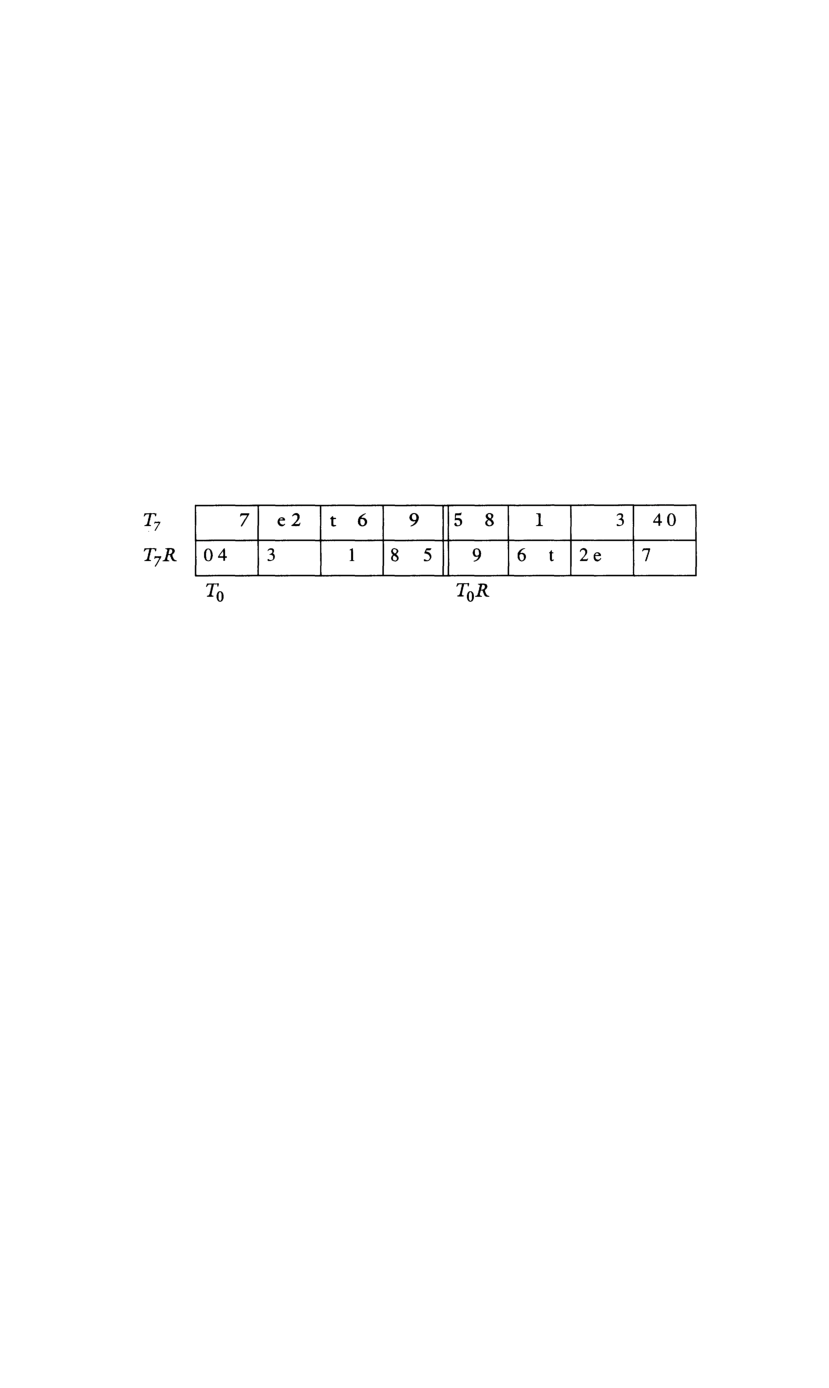
\includegraphics[width=5in]{figures/scotto-array.pdf}
		\caption[Self-derived row in Scotto's \emph{Tetralogy}]{Self-derived row in Scotto's \emph{Tetralogy}.}
    	\label{fig:scotto-array}
	\end{figure}
	
	\noindent Similarly to Ex.~\ref{self-folded}, we can fold the above matrix in order to obtain subsequent levels of derivation. Unlike Ex.~\ref{self-folded}, however, Scotto derives a rotated transform of $S$ from $\R\T_7(S)$. The rows in Fig.~\ref{fig:scotto-folded} are thus $\T_2(S), \R\T_2(S), \rho_6\R\T_2(S)$ and $\rho_6\T_2(S)$, where $\rho$ is the cyclical rotation operator.
	
	\begin{figure}[htbp]
    	\centering
		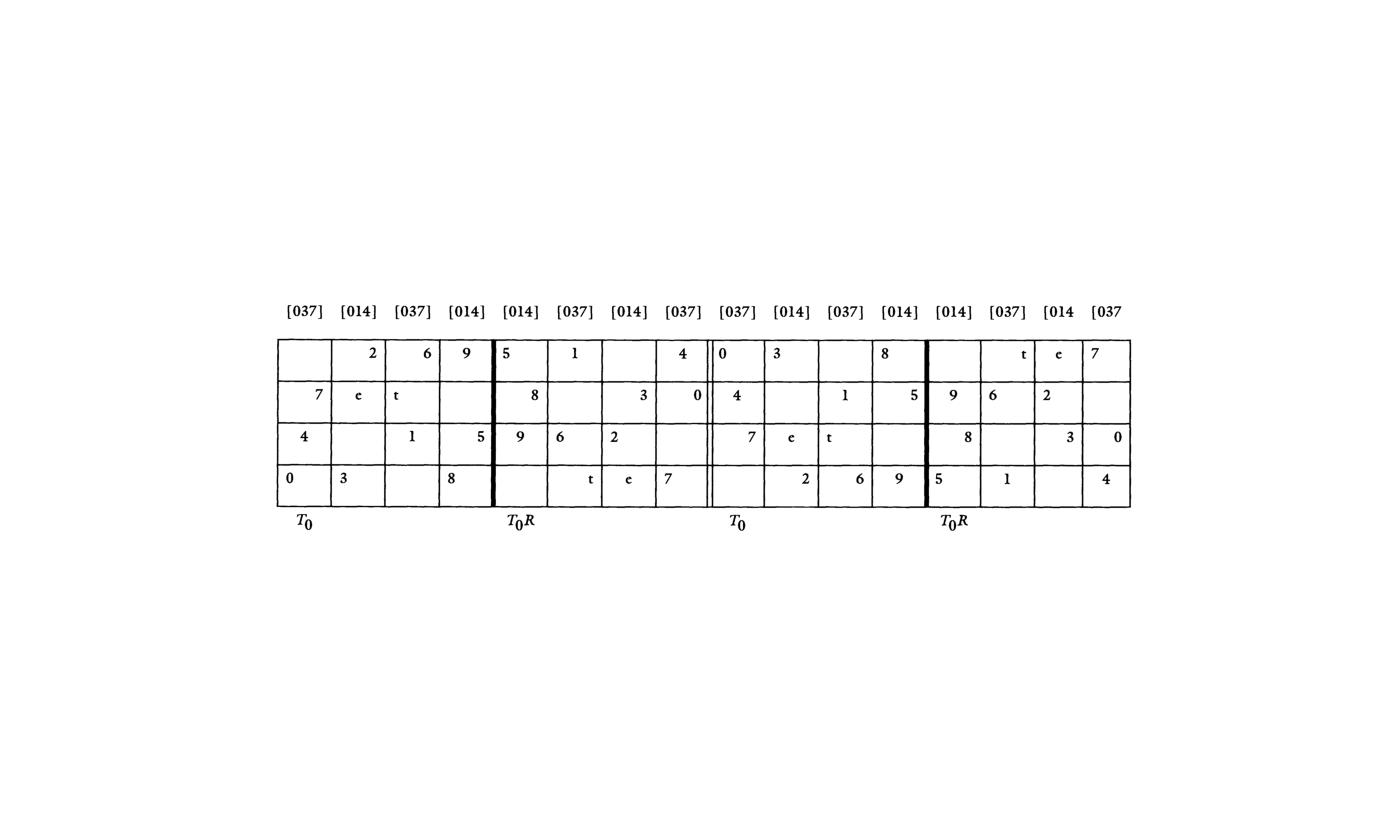
\includegraphics[width=6.5in]{figures/scotto-folded.pdf}
		\caption[Folded derivation in Scotto's \emph{Tetralogy}]{Folded derivation in Scotto's \emph{Tetralogy}.}
    	\label{fig:scotto-folded}
	\end{figure}
	
	\noindent In an entirely Schenkerian fashion, Scotto utilizes the folded array as the source material for the middle-ground structure of \emph{Tetralogy}. The only difference between the derivation array and the Schenkerian graph is that the $\T_2(S)$ now corresponds to the alto register, as seen in Fig.~\ref{fig:scotto-schenker1}. One of the foreground realizations of the Schenkerian graph in Fig.~\ref{fig:scotto-schenker1} is given in Fig.~\ref{fig:scotto-music1}. Rather than a strict serial composition, \emph{Tetralogy} employs a variety of prolongation procedures which are in line with its Schenkerian orientation, but unfortunately beyond the scope of this discussion.
	
	\begin{figure}[htbp]
    	\centering
		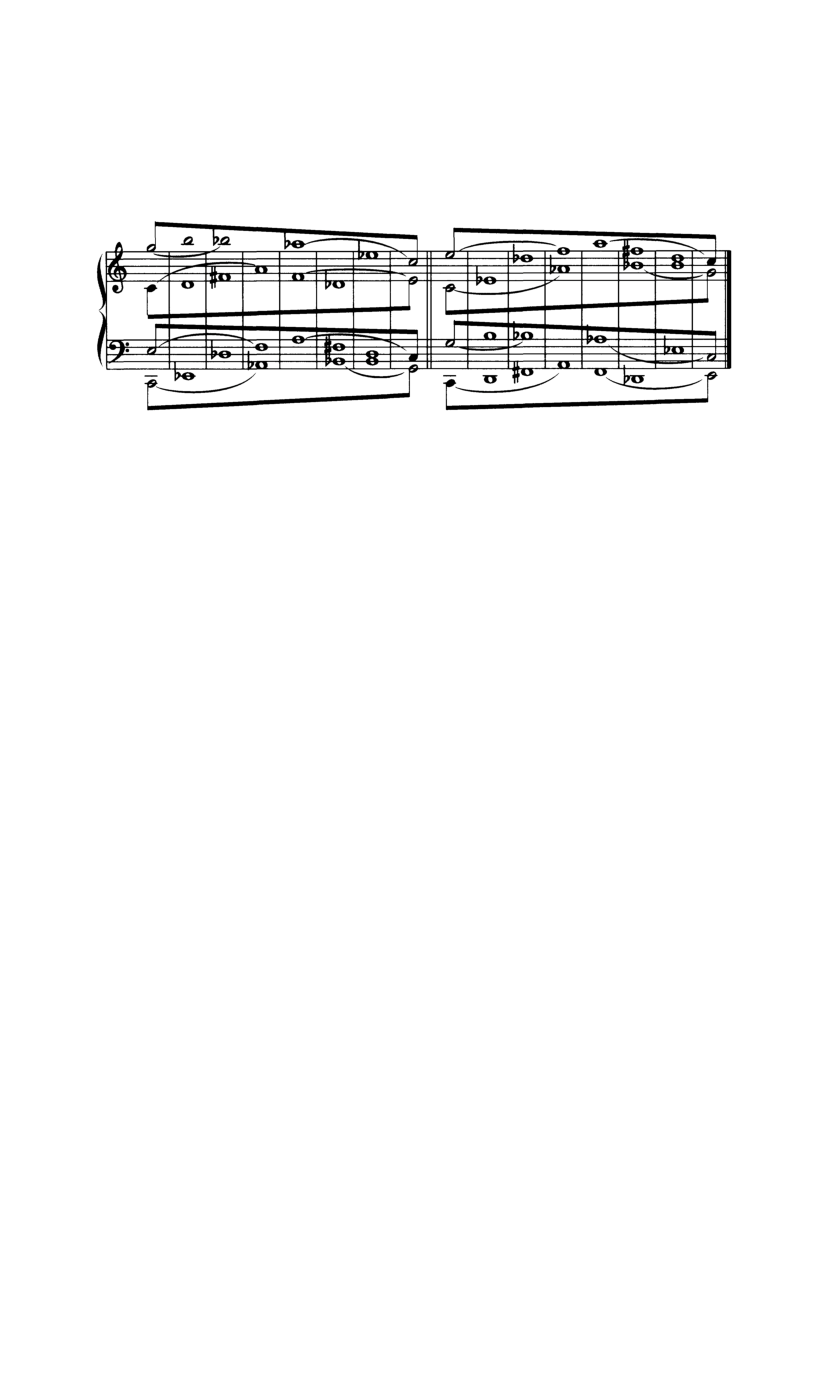
\includegraphics[width=6.5in]{figures/scotto-schenker1.pdf}
		\caption[Schenkerian middle-ground structure in Scotto's \emph{Tetralogy}]{Schenkerian middle-ground structure in Scotto's \emph{Tetralogy}.}
    	\label{fig:scotto-schenker1}
	\end{figure}
	
	\begin{figure}[htbp]
    	\centering
    	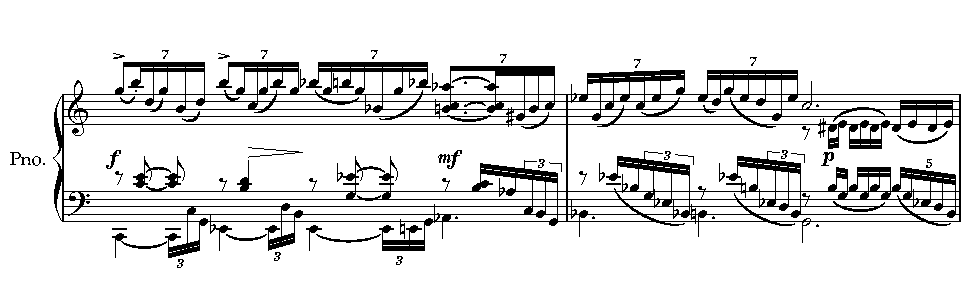
\includegraphics[width=6.5in]{figures/Scotto_1.pdf} %scotto-music1.pdf
		\caption[Musical realization of the middle-ground in Scotto's \emph{Tetralogy}]{Musical realization of the middle-ground in Scotto's \emph{Tetralogy}.}
    	\label{fig:scotto-music1}
	\end{figure}
	
	\begin{figure}[htbp]
    	\centering
    	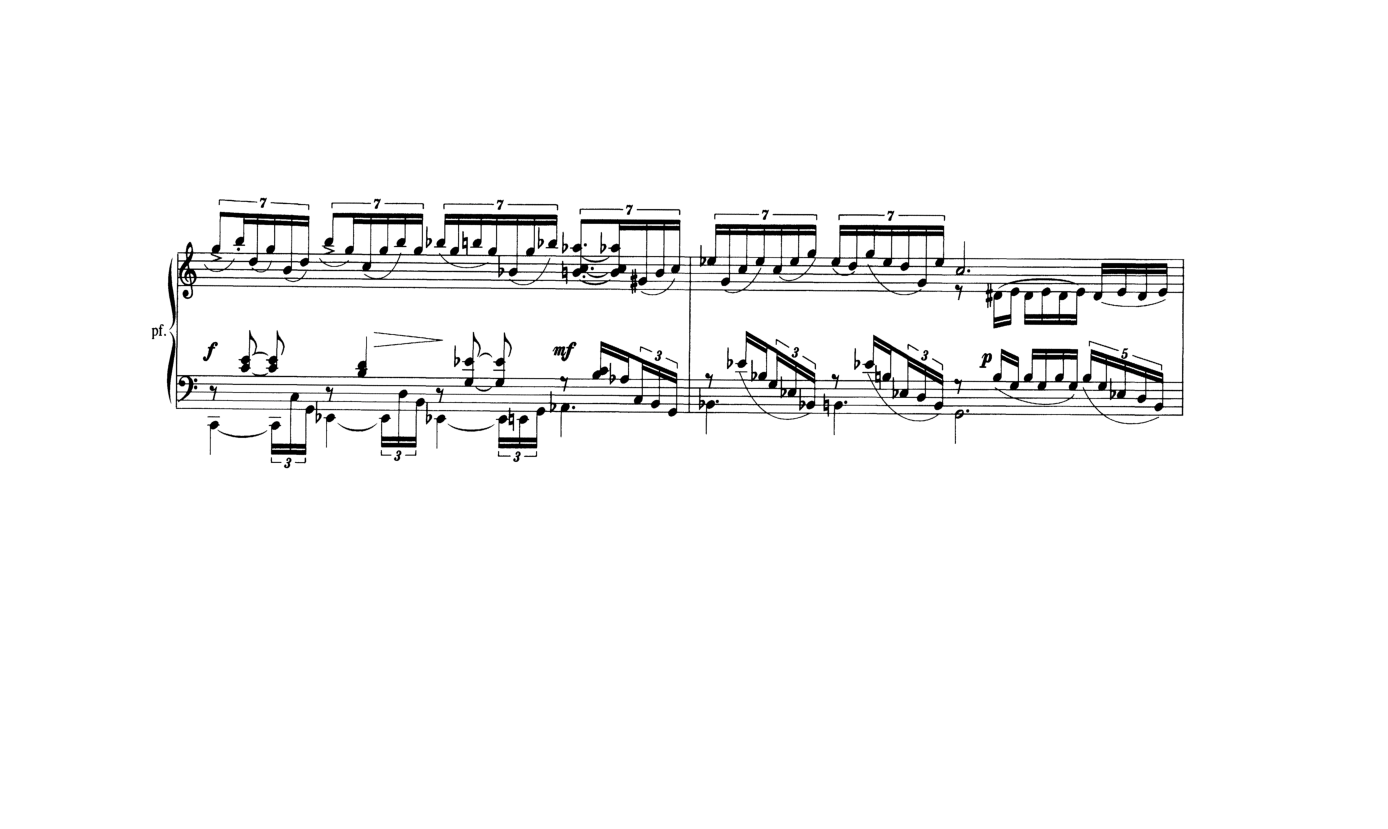
\includegraphics[width=6.5in]{figures/scotto-music1.pdf}
		\caption[Musical realization of the middle-ground in Scotto's \emph{Tetralogy}]{Musical realization of the middle-ground in Scotto's \emph{Tetralogy}.}
    	\label{fig:scotto-music1}
	\end{figure}
	
	\noindent The idea of prolongation in \emph{Tetralogy} extends beyond the foreground musical surface, and is applied as well to the middle-ground structure itself, effectively pushing it further into the background of the piece. The prolongation of the first bar in Fig.~\ref{fig:scotto-schenker1} is depicted in Fig.~\ref{fig:scotto-schenker2}, and a musical realization thereof is displayed in Fig.~\ref{fig:scotto-music2}. 
	
	\begin{figure}[htbp]
    	\centering
    	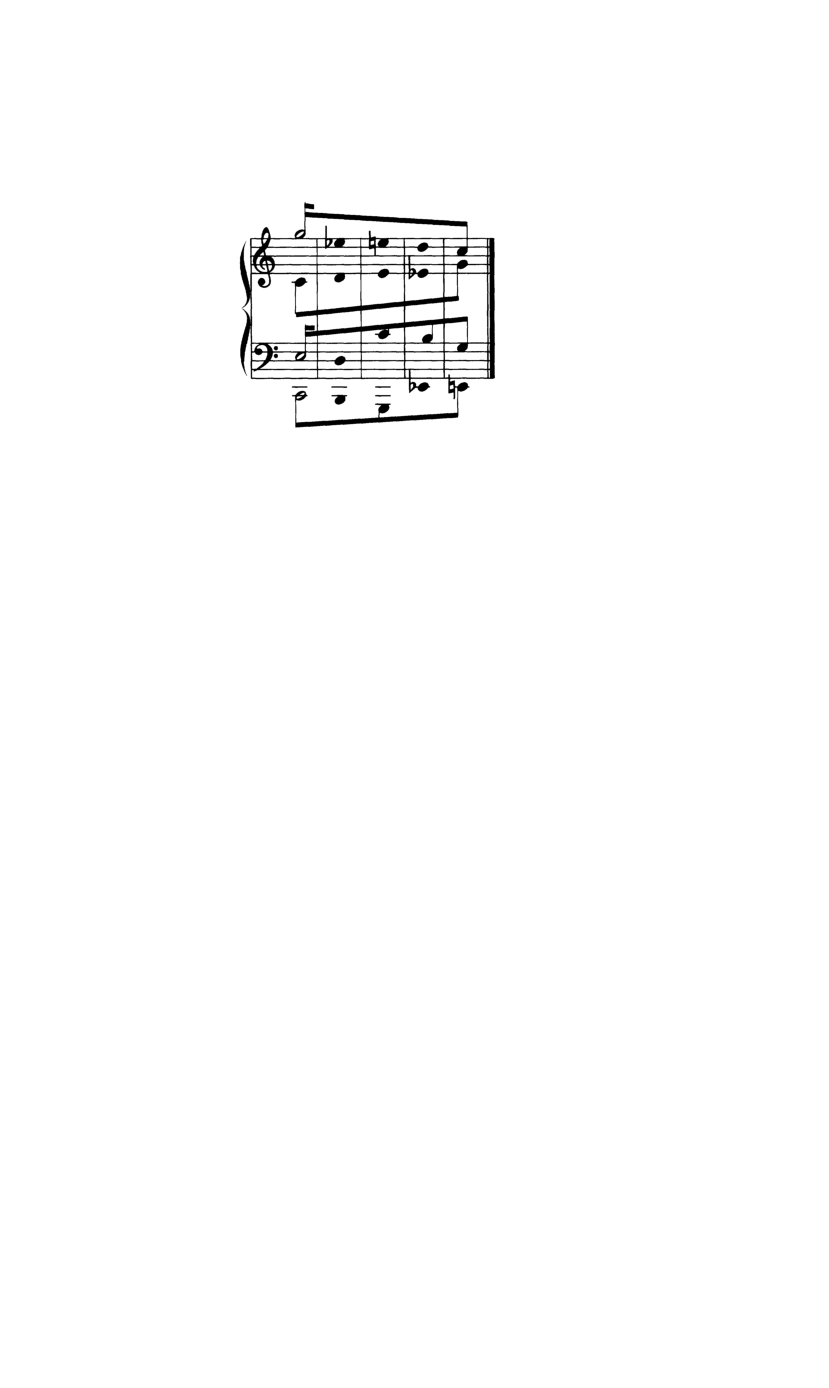
\includegraphics[width=2.2in]{figures/scotto-schenker2.pdf}
    	\caption[Prolongation of the middle-ground structure in Scotto's \emph{Tetralogy}]{Prolongation of the middle-ground structure in Scotto's \emph{Tetralogy}.}
    	\label{fig:scotto-schenker2}
	\end{figure}
	
	\begin{figure}[htbp]
    	\centering
    	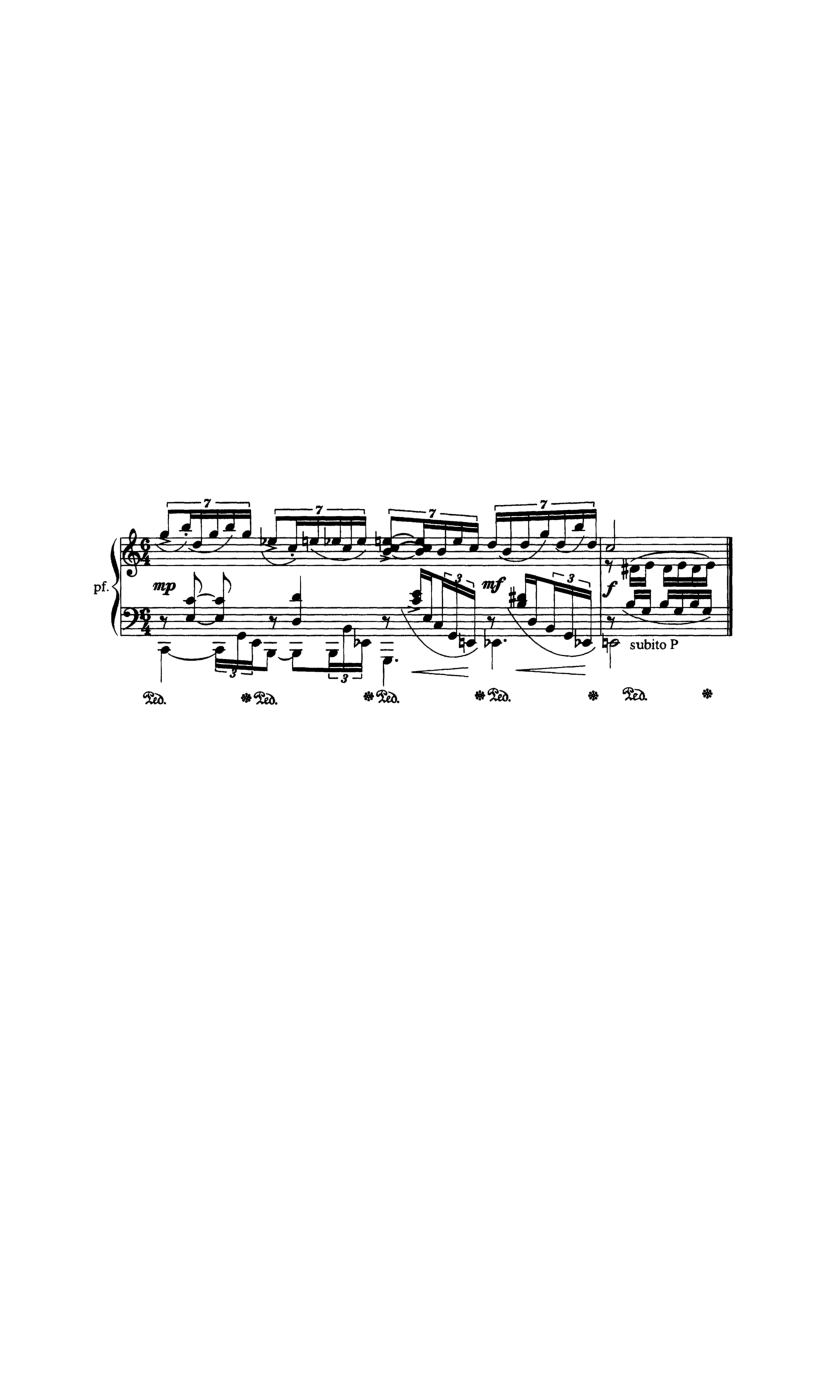
\includegraphics[width=6.5in]{figures/scotto-music2.pdf}
    	\caption[Musical realization of the prolonged middle-ground in Scotto's \emph{Tetralogy}]{Musical realization of the prolonged middle-ground in Scotto's \emph{Tetralogy}.}
    	\label{fig:scotto-music2}
	\end{figure}

\end{example}

The only algorithm that currently exists to find self-derivation matrices is brute force, that is, by trial and error. One must often compose the row while trying to derive a transform of the row itself in a matrix. Self-derivation is the absolute primary concern of this paper, especially because there is so little we know about it. Self-derivation is what makes an order number in a row have multiple functions. Other types of derivation are also important as compositional tools, but they are ultimately special cases of the more constrained type, which is that of self-derivation matrices. In other words, we shall make our priority to investigate the existence of a self-derived matrix for any given row in all generality, that is, for arbitrary $n$-tone equal temperament systems. We shall then devise a general algorithm to obtain such matrices if they exist, as well as investigate how many such matrices do exist for any particular choice of equal temperament system. We shall finally confront our findings with the results in \cite{Kowalski1987b}, which uses a brute force algorithm to compute self-derived rows of a few particular types in the 12-TET. For generalized results, there will be nothing with which to compare, as this territory remains, to this day, mostly uncharted.

%--------------------------------------------------------------------------
\subsection{Derivation from Aggregate Realizations}

The remainder of this chapter will be devoted to exposing derivation matrices that do not necessarily involve the retrograde, then exploring the concept of Mallalieu-type rows, which represent a very peculiar class of self-deriving rows. Mallalieu rows are somewhat better understood in the 12-TET than general derivation, and have many beautiful compositional applications.

\begin{example}
    \cite[224]{Starr1984}
    Let $S = \{ 0, 1, 7, 2 \} | \{ 10, 9 \} | \{ 11, 4, 8, 5 \} | \{ 3, 6 \}$. Given that we always obtain the complement of a row's first hexachord from its second hexachord, we get the trivial case of hexachordal combinatoriality when we match a row with its retrograde. Such combination matrix will have four columns, because of the way we chose to partition $S$:
    \begin{equation}
        A = \left[
        \begin{array}{c|c|c|c}
        	\{ 0, 1, 7, 2 \} & \{ 10, 9 \} & \{ 11, 4, 8, 5 \} & \{ 3, 6 \} \\
        	\{ 6, 3 \} & \{ 5, 8, 4, 11 \} & \{ 9, 10 \} & \{ 2, 7, 1, 0 \}
        \end{array}
        \right] \enspace.
    \end{equation}
    Now consider the cycles of $\T_{11}\I = (0 \; 11) (1 \; 10) (2 \; 9) (3 \; 8) (4 \; 7) (5 \; 6)$. In particular, the first column of $A$ will comprise the partial order $S_1 \cup \R(S_4)$, and this union will, in turn, map onto its hexachordal complement under $\T_{11}\I$, as it takes precisely one element from each of the operation's cycles, all of which have length two. Since the second column above is the complement of the first, it will also map onto its complement under $\T_{11}\I$. Because the third and fourth columns are mirrors of the first two, we do get hexachordal combinatoriality under $\T_{11}\I$ in every column, that is, for the partial orders $S_1 \cup \R(S_4)$ and $S_2 \cup \R(S_3)$, as well as their retrogrades. We do not get the same result between $S$ and $\T_{11}\I(S)$, that is, the first hexachord of $\T_{11}\I(S)$ is \emph{not} the complement of the first hexachord of $S$. This procedure gives us the matrix $\hat{A}$.
    \begin{equation}
        \hat{A} = \left[
        \begin{array}{c|c|c|c}
        	\{ 0, 1, 7, 2 \} & \{ 10, 9 \} & \{ 11, 4, 8, 5 \} & \{ 3, 6 \} \\
        	\{ 6, 3 \} & \{ 5, 8, 4, 11 \} & \{ 9, 10 \} & \{ 2, 7, 1, 0 \} \\
        	\{ 11, 10, 4, 9 \} & \{ 1, 2 \} & \{ 0, 7, 3, 6 \} & \{ 8, 5 \} \\
        	\{ 5, 8 \} & \{ 6, 3, 7, 0 \} & \{ 2, 1 \} & \{ 9, 4, 10, 11 \}
        \end{array}
        \right] \enspace.
    \end{equation}
    What we basically have above is a sequence of four columnar realizations. We are interested in deriving members of the same row class from each column. As aforementioned, there is no algorithm to accomplish this but brute force, and there is no \emph{a priori} way of knowing whether we will succeed at this moment. So far the best we can do is take the intersection of all columns, or transforms thereof and, if the total order class of the intersection is not empty, that is, if it contains the free aggregate and does not contain any symmetry, then Th.~\ref{starr-theorem} guarantees we will be able to derive representatives of this row class from each column. Let $C_1, C_2, C_3, C_4$ be the four columns of the matrix $\hat{A}$. It follows the row $V = \{ 11, 0, 1, 6, 10, 4, 7, 2, 9, 5, 3, 8 \}$ has the property that $T \in \Toc \{ \Ext[ C_1 \cup \R\T_1\I(C_2) \cup \T_1\I(C_3) \cup \R(C_4) ] \}$. We can therefore derive $[V | \R\T_1\I(V) | \T_1\I(V) | \R(V)]$ from the columns of $\hat{A}$.
    \begin{equation*}
        \left[
        \begin{array}{cccccccccccc|cccccccccccc|c}
            & 0 & 1 &&&& 7 & 2 &&&& && 10 &&&&& 9 &&&&& & \\
            &&& 6 &&&&&&& 3 & & 5 && 8 & 4 & 11 &&&&&&& & \\
            \hline
            11 &&&& 10 & 4 &&& 9 &&& &&&&&&&&&&& 1 & 2 & \\
            &&&&&&&&& 5 && 8 &&&&&& 6 && 3 & 7 & 0 && & 2
        \end{array}
        \right. \cdots
    \end{equation*}
    \begin{equation}
        \cdots \left.
        \begin{array}{c|cccccccccccc|cccccccccccc}
            & &&&&&&& 11 & 4 & 8 && 5 && 3 &&&&&&& 6 &&& \\
            & &&&&& 9 &&&&& 10 & &&&&& 2 & 7 &&&& 1 & 0 & \\
            \hline
            & && 0 & 7 & 3 && 6 &&&&& & 8 && 5 &&&&&&&&& \\
            2 & 2 & 1 &&&&&&&&&& &&&& 9 &&& 4 & 10 &&&& 11
        \end{array} \right] \enspace.
    \end{equation}
\end{example}

One of the problems that come with the brute force approach is that, not only is it expensive, but it is ultimately counter-intuitive. It is the same as betting on random numbers on a lottery ticket and asking ourselves whether we have won. We can look in the newspaper after the draw, but that does not increase our odds of winning at all. However, that is exactly what happens when we come up with a series out of sheer guesswork, then ask ourselves whether that series would produce some interesting derivation array. What we want is to be able to increase our odds, to somehow figure out what the winning numbers are. Luckily, this is not the lottery, and the process is certainly not random, so there must be a way to tell exactly how to put together arrays like these without any guessing whatsoever. A partial solution to this problem exists when we use some operation's cycles as building blocks for the columnar aggregates in a derivation matrix.

\begin{example}
    \cite[224]{Starr1984}
    Let $S = \{ 0, 1, 7, 2 \} | \{ 10, 9, 11, 4 \} | \{ 8, 5, 3, 6 \} = S_1 | S_2 | S_3$ and consider the matrix $A = [S | \T_4(S) | \T_8(S)]^T$.
    \begin{equation}
        A = \left[
        \begin{array}{cccc|cccc|cccc}
        	0 & 1 & 7 & 2 & 10 & 9 & 11 & 4 & 8 & 5 & 3 & 6 \\
        	4 & 5 & 11 & 6 & 2 & 1 & 3 & 8 & 0 & 9 & 7 & 10 \\
        	8 & 9 & 3 & 10 & 6 & 5 & 7 & 0 & 4 & 1 & 11 & 2
        \end{array}
        \right] \enspace.
    \end{equation}
    Now let $V$ be in the total order class of the first columnar aggregate of $A$. Next, rewrite the first columnar aggregate of $A$ as the aggregate realization $A_1$.
    \begin{equation}
        A_1 = \begin{tikzcd}
            & 0 \arrow[dr] && 1 \arrow[dr] && 7 \arrow[dr] && 2 \arrow[dr] & \\
            * \arrow[r] \arrow[dr] \arrow[ur] & 4 \arrow[r] & * \arrow[r] \arrow[dr] \arrow[ur] & 5 \arrow[r] & * \arrow[r] \arrow[dr] \arrow[ur] & 11 \arrow[r] & * \arrow[r] \arrow[dr] \arrow[ur] & 6 \arrow[r] & * \\
            & 8 \arrow[ur] && 9 \arrow[ur] && 3 \arrow[ur] && 10 \arrow[ur] &
        \end{tikzcd}
    \end{equation}
    When we see the first column of $A$ as an aggregate realization, it becomes clearer that any $V \in \Toc(A_1)$ must be a succession of augmented triads, say, $V = \{ 4, 8, 0, 9, 1, 5, 11, 7, 3, 2, 10, 6 \}$. We know we are able to linearize $V$ from $A_1$, but the question we should be asking at this point is whether we can linearize some transform of $V$ from the other columns of $A$. The answer depends on the chosen operation, $\T_4$ in this case, and on the chosen $S$. To verify that $A_2$ is a transform of $A_1$, it suffices to check whether there is a base-four $\R\T_n\M\I$ operation that maps $S_1 \pmod 4$ onto $S_2 \pmod 4$. This is easily verified, as indeed
    \begin{equation}
        S_1 \pmod 4 = \{ 0, 1, 3, 2 \} = \T_2\I(\{ 2, 1, 3, 0 \}) = \T_2\I \circ S_2 \pmod 4 \enspace.
    \end{equation}
    The above method works because the elements in each of $A_1$'s columns are incomparable, so we pick from within each column in any order we want. In other words, we could flip $A_1$ horizontally, say, and still have the same aggregate realization. Since we can reduce all of $A$'s columns $\mod 4$ by construction, it becomes enough to only consider each column's residue modulo four, and four-tone operations. Since $S_1 \pmod 4 = S_3 \pmod 4$, we can derive $V$ itself from $A_3$, and thus obtain the following derivation matrix, where the second column is $\T_2\I(V)$:
    \begin{multline}
        \left[
        \begin{array}{cccccccccccc|cccccc}
        	&& 0 && 1 &&& 7 && 2 && & 10 &&&&& 9 \\
        	4 &&&&& 5 & 11 &&&&& 6 & && 2 && 1 & \\
        	& 8 && 9 &&&&& 3 && 10 & & & 6 && 5 &&
        \end{array}
        \right. \cdots \\\\
        \cdots \left.
        \begin{array}{cccccc|cccccccccccc}
        	&& 11 && 4 & & & 8 &&&& 5 &&& 3 &&& 6 \\
        	3 &&&&& 8 & && 0 & 9 &&&& 7 &&& 10 & \\
        	& 7 && 0 && & 4 &&&& 1 && 11 &&& 2 &&
        \end{array}
        \right] \enspace.
    \end{multline}
    It would be rather undesirable, however, that we should be restricted to rows that are merely the concatenation of cycles from an operation. We can certainly use the machinery hitherto developed to evaluate what other rows can be derived from $A$. Knowing that the columns of $A$ are related as aggregate realizations by the operation tuple $\mathcal{A} = [\T_0 \; \T_2\I \; \T_0]$, we can regard the $A_i$ as columnar aggregates, then take $\hat{A} = \Ext[\bigcup_i(\mathcal{A}_i \circ A_i)]$. By Th.~\ref{starr-theorem}, any row we are able to linearize from $\hat{A}$, will be in $\bigcap_i \Toc(A_i)$, and thus we can derive its $\mathcal{A}_i$-transform from each $i$-column of $A$. Below is the columnar aggregate $\hat{A}$.
    \begin{equation}
        \hat{A} = \begin{tikzcd}
            & 0 \arrow[r] \arrow[ddr] & 1 \arrow[r] \arrow[dr] & 7 \arrow[r] \arrow[ddr] & 2 \arrow[dr] & \\
            * \arrow[r] \arrow[dr] \arrow[ur] & 4 \arrow[r] \arrow[ur] & 5 \arrow[r] \arrow[dr] & 11 \arrow[r] \arrow[ur] & 6 \arrow[r] & * \\
            & 8 \arrow[r] \arrow[ur] & 9 \arrow[r] \arrow[uur] & 3 \arrow[r] \arrow[ur] & 10 \arrow[ur] &
        \end{tikzcd}
    \end{equation}
    It follows $\hat{V} = \{ 0, 1, 4, 8, 9, 5, 7, 2, 11, 3, 10, 6 \}$ can be linearized from $\hat{A}$, yielding the derivation matrix below:
    \begin{multline}
        \left[
        \begin{array}{cccccccccccc|cccccc}
        	0 &&&& 1 & 7 &&& 2 &&&&&&& 10 && \\
        	&&& 4 &&& 5 & 11 &&& 6 && 2 &&&& 1 & \\
        	& 8 & 9 &&&&&&& 3 && 10 && 6 & 5 &&& 7
        \end{array}
        \right. \cdots \\\\
        \cdots \left.
        \begin{array}{cccccc|cccccccccccc}
        	9 &&& 11 && 4 && 8 &&&&& 5 &&& 3 & 6 & \\
        	& 3 &&& 8 && 0 && 9 &&& 7 &&&&&& 10 \\
        	&& 0 &&&&&&& 4 & 1 &&& 11 & 2 &&&
        \end{array}
        \right] \enspace.
    \end{multline}
\end{example}

%--------------------------------------------------------------------------
\section{Final Remarks}

We now devote our attention to summarizing the theoretical objectives of this research. The main motivation is to understand the construction of self-derivation precisely, that is, for any given row, whether it is capable of producing any known form of self-derivation. Conversely, given some self-derivation procedure, we would like to be able to provide a complete description of the class of rows that participate therein. All the above shall be done in all generality, that is, for arbitrary $n$-tone temperament systems. After having dealt with the more constrained case of self-derivation, we shall attempt to extend the above ideas to the general derivation setting, id est, without the requirement that the derived row be in the same row class as the originating row. General derivation is less strict and better understood than self-derivation, but lacks the latter's potential for cohesiveness. Whatever is already present in the literature, shall be extended to other equal temperament systems than the 12-TET. We shall also attempt to describe how specific patterns of derivation arise. In other words, given a pattern of order numbers, for what rows, and under which operations, do we get known forms of derivation and self-derivation. Analogously, we would like to investigate how chains of pitch-class operations are induced by derivation procedures, as to determine how a piece may be composed from the standpoint of its syntax, perhaps even prior to establishing any compositional surface. Many well-known derivation procedures described in this chapter also lack a more rigorous treatment. We shall make precise, providing proofs when necessary, what the constraints regarding the choice of operation are for folded and shifted derivations. In particular, we will investigate the need for commutativity, as well as determine which of the aforementioned forms support derivation matrices that do not involve the retrograde. We shall also take into account the role of the cyclic rotation operator, particularly in what regards folded self-derivations. Cyclic rotation and its invariances will be intimately connected with our combinatorial findings (in the mathematical sense). We shall make use of known brute-force algorithms, such as \cite{Kowalski1987b}, to confront our findings, and also verify their correctness if appropriate. Finally, we will generalize mallalieu-type rows to arbitrary equal temperament systems, giving a precise count and description of their untransposed representatives. In addition, we will investigate generalizations of the mallalieu property by relaxing the requirement that we get a copy of the row at every single index, as proposed in \cite{Mead1989}. We shall also investigate whether transposition is the only operation that affords the mallalieu property.

Our theoretical framework will be purely mathematical, with the sole exception of a few brute-force algorithms that will be used to guide our findings. As previously discussed, mathematics can greatly simplify our search for answers, and a solid mathematical theory of the musical objects that pertain to this study are a requirement for mature compositional decisions that involve the techniques here discussed. Anticipating, as much as possible, the symmetries of a musical construct of the sort with which we will be concerned can help a composer determine the outlook and feasibility of an entire piece. Mathematics is also crucial for constructing efficient computer algorithms that employ such techniques, and is the only resource we actually have against brute force. Much of the mathematics required by our findings will be mentioned in the theoretical framework, although some basic knowledge is omitted. We assume the reader will have some basic knowledge of abstract algebra, to the extend that many graduate texts in atonal music theory will require. Our treatment shall depart from the concept of group actions. A working knowledge of twelve-tone theory is also required. We assume the reader is familiar with such basic concepts as contour, pitch, and pitch-class spaces, intervals and interval classes, set classes, operations, and associated group-theoretic notions.

The last chapter of the present work will deal with some musical applications of derivation techniques. Given the historical application of these techniques to almost exclusively the pitch domain, and in the interest of shedding new light onto such procedures, the compositional applications we shall describe will have a certain bias toward employing derivation in dimensions other than pitch. Also, given that most examples of derivation in the twentieth-century repertoire are of instrumental music, we shall here pursue the electroacoustic music avenue, with a particular interest in algorithmic processes. Beyond uniqueness and innovation, we justify and motivate our choices by the fact that many of our generalizations, such as, say, constructing a mallalieu row in 50 elements, become problematic, if not incompatible, with instrumental music.
